\documentclass[final,twocolumn,5p]{elsarticle}
\usepackage{tikz}
  \def\firstcircle{(90:1.75cm) circle (2.5cm)}
  \def\secondcircle{(210:1.75cm) circle (2.5cm)}
  \def\thirdcircle{(330:1.75cm) circle (2.5cm)} 
\usepackage{comment}
\usepackage{framed,graphicx}
\usepackage{multirow}
\usepackage{rotating}
\usepackage{amsmath}
\usepackage{bigstrut}
\usepackage{color}
\usepackage{graphics} 
\usepackage{eqparbox}
\usepackage{graphics}
\usepackage{colortbl} 
%\usepackage{times}
 \usepackage{mathptmx} \usepackage[scaled=.90]{helvet} \usepackage{courier}
\usepackage{balance}
\usepackage{picture}
\usepackage{algorithm}
\usepackage{algorithmicx}
\usepackage{algpseudocode}
\usepackage[export]{adjustbox}
\renewcommand{\footnotesize}{\scriptsize}
\definecolor{lightgray}{gray}{0.8}
\definecolor{darkgray}{gray}{0.6}
\definecolor{lavenderpink}{rgb}{0.98, 0.68, 0.82}
\definecolor{celadon}{rgb}{0.67, 0.88, 0.69}
\renewcommand{\algorithmicrequire}{\textbf{Input:}}
\renewcommand{\algorithmicensure}{\textbf{Output:}}
%%% graph
\newcommand{\crule}[3][darkgray]{\textcolor{#1}{\rule{#2}{#3}}}

\newcommand{\quart}[4]{\begin{picture}(80,4)%1
{\color{black}\put(#3,2){\circle*{4}}\put(#1,2){\line(1,0){#2}}}\end{picture}}

\definecolor{Gray}{gray}{0.95}
\definecolor{LightGray}{gray}{0.975}

\newcommand{\wei}[1]{\textcolor{red}{Wei: #1}} 
\newcommand{\Menzies}[1]{\textcolor{red}{Dr.Menzies: #1}} 

%% timm tricks
\newcommand{\bi}{\begin{itemize}[leftmargin=0.4cm]}
\newcommand{\ei}{\end{itemize}}
\newcommand{\be}{\begin{enumerate}}
\newcommand{\ee}{\end{enumerate}}
\newcommand{\tion}[1]{\S\ref{sect:#1}}
\newcommand{\fig}[1]{Figure~\ref{fig:#1}}
\newcommand{\tab}[1]{Table~\ref{tab:#1}}
\newcommand{\eq}[1]{Equation~\ref{eq:#1}}


\usepackage[shortlabels]{enumitem}  
\usepackage{url}

\usepackage{tikz}
\usepackage{xcolor}
   \usepackage[framed]{ntheorem}
\usepackage{framed}
\usetikzlibrary{shadows}
%\newtheorem{Lesson}{Lesson}
\theoremclass{Lesson}
\theoremstyle{break}

% inner sep=10pt,
\tikzstyle{thmbox} = [rectangle, rounded corners, draw=black,
  fill=Gray!20,  drop shadow={fill=black, opacity=1}]
\newcommand\thmbox[1]{%
  \noindent\begin{tikzpicture}%
  \node [thmbox] (box){%
\begin{minipage}{.94\textwidth}%    
      \vspace{-3mm}#1\vspace{-3mm}%
    \end{minipage}%
  };%
  \end{tikzpicture}}

\let\theoremframecommand\thmbox
\newshadedtheorem{lesson}{Research answer}
 
 

\begin{document}

\begin{frontmatter}

\title{Which ``Bad Smells'' Can Be Ignored?}

\author{Rahul Krishna\corref{cor1}\textsuperscript{a,}}
\ead{rkrish11@ncsu.edu}
\author{Tim Menzies\corref{cor1}\textsuperscript{a,}}
\ead{tim.menzies@gmail.com}
\author{Lucas Layman\textsuperscript{b}}
\ead{ llayman@cese.fraunhofer.org }
\cortext[cor1]{Corresponding author: Tel:+1-919-396-4143(Rahul)}
\address{\textsuperscript{a}Department of Computer Science, North Carolina State University, Raleigh, NC, USA\\
\textsuperscript{b}Fraunhofer CESE, College Park, USA}

\begin{abstract} 
{\bf Context: }The literature lists many bad smells that may be detrimental to a software system. But which are relevant to the current project and which can be ignored?
Developers, text books, and tools disagree on which bad smells are important. 
Further, it is unclear at what threshold values smell-related metrics
should trigger code improvement or preventative maintenance. Most studies do not offer {\em both} measurable metrics {\em and} a threshold for their proposed bad smells.

\noindent 
{\bf Objective: }We seek to propose a tool to prioritize  bad  smells.

\noindent
{\bf Method: } We introduce XTREE, a tool which, given a historical log of defects seen previously in the code, deprioritizes bad smells that have no prior association with defects. 

\noindent
{\bf Evaluation: } We evaluate XTREE's recommendations for bad smell improvement against recommendations from previous work (Shatnawi, Alves, and Borges) using multiple data sets of code metrics and defect counts.  

\noindent
{\bf Results: }Code modules that are changed in response to XTREE's recommendations contain significantly fewer defects than recommendations in previous studies. Further, XTREE endorses changes to far fewer code metrics, and that bad smell recommendations (learned from previous studies) are not universal to software projects.

\noindent
{\bf Conclusion: }It is important to  prioritize the importance of specific bad smells in the context of each project since not all bad smells are relevant to the current project. Based on these results, we endorse using bad smells to guiding refactoring. 

\end{abstract}
\end{frontmatter}
\pagenumbering{arabic} %XXX delete before submission

\vspace{1mm}
\noindent
{\bf Keywords:} Bad smells,
performance prediction,  decision trees 


\section{Introduction}

\noindent
According to   Fowler ~\cite{fowler99}, bad smells (a.k.a. code smells)
are ``a surface indication that usually corresponds to a deeper problem''.
Fowler strongly recommends   removing   code smells   by
\begin{quote}
``...applying a series of small behavior-preserving transformations, each 
of which seem ``too small to be worth doing''. 
The  effect of   these transformations is quite significant. By doing them in small steps you {\em reduce the risk of introducing errors}'' (our italics).
\end{quote}
The literature is divided on the merits of bad smells.
Much research endorses them to guide
code improvement (e.g., refactoring or preventative maintenance). A recent literature review by Tufano et al.~\cite{Tufano2015}  
lists dozens of papers on smell detection and repair tools. 

Other papers cast doubt on the value of bad smells
as triggers for code improvement~\cite{Mantyla2004,Yamashita2013,Sjoberg2013}. 
As we show in this paper,  
 tools, text books, and developers disagree on what bad smells
are important enough to hunt down and eliminate. Our findings
are consistent with other research suggesting that universal bad
smells that ignore project context are not useful to guide refactoring~\cite{Mantyla2004,Yamashita2013,Sjoberg2013}.


Bad smells are a widely used technique for evaluating code. As of  early 2016, ACM Digital Library reports 
the Fowler text has 6434 references. A search  on {\em ``bad smell''programming} 
where {\em proceedings=ICSE} finds 1,748 papers since 2006.
Hence it is important to understand the value of
this popular topic.  
Valuable development resources may be wasted on bad smells that are ``bad''; i.e. 
 irrelevant or misleading
for some particular project.

To address this problem, we propose the XTREE
tool that uses: 
     \begin{itemize}
         \item A historical log of defects seen previously in the code;
         \item  Bad smells expressed in terms of the 
          metrics   in that log;
         \item Some proposed refactorings justified using those bad smells.
     \end{itemize}
Given that,  XTREE can determine which
  proposed refactorings are to be ignored
since they are not justifiable  
with respect to the history of the project. XTREE addresses four problems that  make it hard to  learn useful
bad smells for a particular project.

{\em PROBLEM \#1:} As discussed in the next section, programmer
  cognitive biases result in different
developers declaring that
bad smell X or Y is most important. 
 XTREE offers a way to assess the value of competing recommendations to address smell X vs. Y.
  

{\em PROBLEM \#2:} Not all bad smells can be fixed. 
When new code must
be combined with code from a third party, 
sometimes the constraints of that code 
lead unavoidably to bad smells violations (e.g.
developers might need to passed as a single closure a  very long method
to  a third-party GUI toolkit).   In this case,
a refactoring proposed to reduce that bad smell
may be irrelevant since it cannot be applied to this code base.

To address this problem, XTREE {\em reasons optimistically} to find the set
$R_0$ of refactorings that \textit{might} be useful (see \tion{rq} on optimistic reasoning).
The space of \textit{actually usable} refactorings is 
the subset $R_1 \subseteq R_0$.
If a developer's proposed refactoring $R_2$ is
not in $R_0$, then it cannot be in the usable
set $R_1$.  We show experimentally that XTREE
often recommends small subsets of
code metrics as useful guides for refactoring. Thus, we
can rule out some proposed refactorings
since many of those proposals fall outside of the space
useful refactorings ($R_0$) suggested by XTREE.  



{\em PROBLEM \#3:}  
Shantnawi~\cite{Shatnawi10} warns most  studies do not offer
{\em both} a metric and a threshold for proposed bad smells. For example,  Darcy and Kemerer~\cite{darcy05}
discuss object-oriented (OO) design metrics that might defect bad smells (e.g. an excessive
depth of inheritance tree), but they do not define thresholds
for when the code starts to smell bad.  
Shatnawi~\cite{Shatnawi10}
and  Alves et al.~\cite{Alves2010} are rare cases where both metrics and thresholds are defined (see \tion{bst}).
However, their approaches do not explore the interconnections between sets of code metrics. This is important if sets of
code metrics have to be changed at the same time.
For example, it is not possible to refactor a
long method if several smaller ones without increasing
the coupling metrics of a class. 
More generally, we say that bad smell thresholds should be
{\em conjunctions} of metric+threshold pairs that need to be changed {\em together}.
Shatnawi~\cite{Shatnawi10}
and Alves et al. report {\em disjunctions} of multiple metrics+thresholds~\cite{Shatnawi10,Alves2010} without indicating how changes to these metrics are related.



To address this third problem, 
XTREE   generates {\em conjunctions} of   thresholds
than should  be considered at the same time.

 
{\em PROBLEM \#4:} It is hard to judge the  effects of removing bad smells.
Refactored code cannot be assessed just by a rerun of the the test
suite (since refactorings are supposed to preserve behavior), and otherwise one must wait for new defect reports to evaluate the effect of refactoring changes on code.  
% waiting to observe 
% code refactorings is meant to
% preserve the behavior of the system (i.e. the same tests
% should pass before and after the refactoring). 
% Also, it many not be practical
%  to assessing refactorings by making the
% refactorings,  then seeing what happens to that code for the rest
% of the project. In a test-driven agile project, as
% SCRUM meetings change what stories are implemented next,
% the operational profile that lead to defects in the old
% code may not be repeated in future executions. 
To resolve this  problem, SE researchers such as 
Cheng et al.~\cite{Cheng10}, O'Keefe et al.~\cite{OKeeffe08,OKeeffe07},
Moghadam~\cite{Moghadam2011} and Mkaouer et al.~\cite{Mkaouer14}
use a pair of systems: 
\begin{enumerate}
    \item One system to propose changes;
\item A separate system to assess
how defective is the code before and after some
refactoring.
\end{enumerate}
For the second system,
 Cheng, O'Keefe, Moghadam and  Mkaouer et al. use the QMOOD hierarchical
quality model~\cite{Bansiya02}.
A shortcoming of QMOOD
is that quality models learned from other projects
may perform poorly when applied to new projects~\cite{localvsglobal}.


To solve this fourth problem, this study  eschews
older quality models like QMOOD, we use
Random Forests~\cite{Breiman2001} to learn defect predictors
from OO code metrics.
Note that, unlilke QMOOD, such measurements 
  are specific to the project, and the measurements can be reconstructed and the predictors rebuilt for other projects.
  
 
 
The rest of this paper is structured as follows. 
The next section
discusses the cognitive
biases that make developers disagree on the relevance of those bad smells to
their particular projects
(that discussion is our motivation for developing 
tools like XTREE). This is followed by a discussion
on various methods to learn thresholds for bad smells.
After evaluating those methods, we discuss various threats to
validity that threaten our conclusions.


Before  that, we offer one following note on a
core assumption of XTREE.
XTREE   is focused on Fowler's bad smells
as contributors to software defects. Some researchers 
 suggest that discussing bad smells is useful for more just reducing defects. For example, Bosu and Carver~\cite{bosu13} report that
debates about code smells and refactorings can (a)~introduce new comers to the code base or (b)~share knowledge on a team
about interactions within the code. In that view, 
the concept of refactoring can be useful
even if it does not address issues of defects. 


\subsection{Contributions of this Paper }
The XTREE learner has not been reported
previously. 
The comparative analysis of XTREE
    versus previously published approaches to learning
    bad smell detectors shows
    that XTREE   rarely perfoms
      worse that the other approaches~\cite{Shatnawi10,Alves2010}
      and often is it   much better at proposing
      changes that reduce the expected
      number of of the defects. Further, the number
    of code metrics mentioned by XTREE is far
    fewer than other approaches, making it easier to validate refactorings proposed by
    developers. 
We
show here that XTREE is less verbose and offers better recommendations than the CD tool   developed previously with Borges~\cite{me12c}.
 The experimental rig
 used to comparatively assess
    XTREE is another novel contribution\footnote{tiny.cc/XTREE}. Using the design
    of that rig,
    other researchers could confirm/improve/refute
    the conclusions of this paper.
    

 
 
   


\section{Motivation}\label{sect:prelim}

Why build tools like XTREE to  critique proposed developer actions?
Are not those developers the best guide to what is important or irrelevant
to their code? Developer {\em cognitive biases} can mislead them to
assert that some things are important and relevant when they are not.
This section discusses those biases-- firstly in the general sense
across all SE beliefs; then secondly in the   context of code smells.

A widespread malaise in software engineering is that
beliefs about software are rarely revised and hence may be
  inaccurate and 
misleading~\cite{passos11,jorgensen09,mei15,me16phase,prem16}. Software developers may have strong views on many issues, including bad smells, but those views may be wrong for the current
project.
Software engineering is not the only field with this problem.
  For example, the medical profession applies many practices based on studies that have been disproved (a recent article in the Mayo Clinic Proceedings~\cite{prasad13} found 146 medical practices based on studies in year i, but which were reversed by subsequent trials within years i + 10). Even when the evidence for or against a treatment or intervention is clear, medical providers and patients may not accept it~\cite{aschwanden10}. Aschwanden warns that {\em cognitive biases} such as confirmation bias (the tendency to look for evidence that supports what you already know and to ignore the rest) influence how we process information~\cite{aschwanden15}.

As in medicine, so too in software engineering.
According to Passos et al.~\cite{passos11},  developers often  assume that the lessons they learn from a few past projects are general to all their future projects. They comment ``past experiences were taken into account without much consideration for their context''~\cite{passos11}.  J{\o}rgensen \& Gruschke~\cite{jorgensen09} offer a similar warning. They report that the supposed software engineering ``gurus'' rarely use lessons from past projects to improve their future reasoning and that such poor past advice can be detrimental to new projects.~\cite{jorgensen09}. Other studies have shown some widely-held views are   now questionable given new evidence:

\begin{enumerate} 
% COMMENT FROM LL: This bullet is weak. Maybe goto isn't used in an unrestricted manner because of Djikstra's warning.
% \item
% Nagappan et al. analyzed~\cite{mei15} 
% how   {\tt goto}  was used  in 11,000 Github repositories. 
% They found that developers
% rarely used {\tt goto} in the unrestricted manner that alarmed Dijkstra in his  1968
% memo ``Go to statement considered harmful''~\cite{Dijkstra68}.
\item
In other work~\cite{me16phase} with the Software Engineering Institute (SEI), we have revisited
the ``phase delay'' truism that {\em the cost of fixing an error dramatically increases the longer it is in the system}. 
We found no evidence for such large   phase delay effect in modern
software (in 171 software projects shepherded
by the SEI, 2006-2014) possibly since it has been  heavily mitigated by $21^{st}$ century software development languages, tools and development practices. 
Whatever the reason, the main point  is that phase delay is a widely
held belief, despite little recent evidence to support it.
\item
Devanbu et al.  examined responses from 564 Microsoft software developers from around
the world, they found that  ``(a)~programmers do indeed have very
strong beliefs on certain topics; (b)~their beliefs are primarily formed
based on personal experience, rather than on findings in empirical
research; (c)~beliefs can vary with each project, but do not necessarily
correspond with actual evidence in that project''~\cite{prem16}.
\end{enumerate}
Devanbu et al. further  comment that ``programmers give personal experience
as the strongest influence in forming their opinions''. This is a troubling
result, especially given the above comments from Passos and  J{\o}rgensen et al.~\cite{passos11,jorgensen09} about how quickly practitioners form, freeze, and rarely revist those opinions.



\def\checkmark{\tikz\fill[scale=0.4](0,.35) -- (.25,0) -- (1,.7) -- (.25,.15) -- cycle;} 
\begin{figure}[!t] 
\scriptsize
\centering
\begin{tabular}{r|c|c|c|c} 


\begin{turn}{75}Fowler'99~\cite{fowler99} and~\cite{Kerievsky2005}\end{turn} &\begin{turn}{75} Lanza'06~\cite{Lanza2006}\end{turn} & \begin{turn}{75}SonarQube~\cite{sq15} \end{turn} &  \begin{turn}{75}Yamashita'13\cite{Yamashita2013} \end{turn}& \begin{turn}{75} Developer Survey 2015\end{turn}\\\hline
  Alt. Classes with Diff. Interfaces & & & & \\
  Combinatorial Explosion~\cite{Kerievsky2005} & & &  & \\
  Comments & & & 11 & VL\\
  Conditional Complexity~\cite{Kerievsky2005} & & & 14  & ?\\
  Data Class & \checkmark & &  &\\
  Data Clumps &  &  &  &\\
  Divergent Change & & &  & \\
  Duplicated Code & \checkmark & \checkmark & 1  & VH\\
  Feature Envy & \checkmark & & 8  &\\
  
  Inappropriate Intimacy & & \checkmark &  & L\\
  Indecent Exposure~\cite{Kerievsky2005} & & &  & ?\\
  Incomplete Library Class & & &  &\\
  Large Class & \checkmark & \checkmark & 4  & VH\\
  Lazy Class/Freeloader & & \checkmark & 7  &\\
  Long Method & \checkmark& \checkmark & 2  & VH\\
  Long Parameter List &  & \checkmark & 9  & L \\
  
  Message Chains & & &  & H\\
  Middle Man & &  &  &\\
  Oddball Solution~\cite{Kerievsky2005} & & &  & \\
  Parallel Inheritance Hierarchies & & &  &\\
  Primitive Obsession &  & &  &\\
  
  Refused Bequest & \checkmark & \checkmark &  & \\ 
  Shotgun Surgery & \checkmark& &  & \\
  Solution Sprawl~\cite{Kerievsky2005} & & &  &\\
  Speculative Generality & & &  & L\\
  Switch Statements &  & &  & L\\
  Temporary Field & & \checkmark &  & ?\\
  \end{tabular}
%   \multicolumn{5}{l}{} \\
%   \multicolumn{5}{l}{\textsuperscript{\textdagger} + Exact rule, - Possibly related rule} \\
%     \multicolumn{5}{l}{\textsuperscript{\textdaggerdbl} + is included in list} \\
%     \multicolumn{5}{l}{\textsuperscript{\textexclamdown} VH: Very High, H: High, L: Low, VL: Very Low, ?: Still investigating} \\
%   \multicolumn{5}{l}{\textsuperscript{*} Computation is based on more than simple metrics.} \\

\caption{Bad   smells from different sources.  Check marks (\protect\checkmark) denote   a bad smell was mentioned.
Numbers or symbolic labels (e.g. "VH") denote  a priorization comment (and
``?'' indicates lack of consensus). Empty cells
denote some bad smell listed in column one that was not found relevant
in other studies.
Note: there are many blank cells.}
\label{fig:smells}
\end{figure}

If the above remarks hold true for bad smells, then we would expect
to see much disagreement on which bad smells are important and relevant
to  a particular project. This is indeed the case.
The first column of \fig{smells} 
lists  commonly mentioned bad smells and comes from Fowler's 1999 text~\cite{fowler99} and a subsequent 2005 text by Kerievsky that is widely cited~\cite{Kerievsky2005}.
The other
columns show data from other studies on which bad smells matter most.
The columns marked as Lanza'06 and Yamashita'13 are from peer reviewed literature. The column maked SonarQube is a popular open source
code assessment tool that includes detectors for six of the bad smells
in column one. 
The {\em developer survey}   (in the right-hand-side column),
  this shows the results of an hour-long whiteboard sessions with a group of 12 developers from a Washington
    D.C. web tools development company. Participants
    worked in a round robin manner to rank the bad smells they thought were
    important (and any disagreements were discussed with the whole group).
     Amongst the group, there was  some
    consensus on  the priority of which bad smells to fix
    (see the annotations VH=very high,
    H=high, L=low, VL=very low, and ``?''= no consensus).  
   
   
   
\begin{figure*}[t!]
	\renewcommand{\baselinestretch}{0.8}\begin{center}
		{\scriptsize
			\begin{tabular}{c|l|p{4.7in}}
				amc & average method complexity & e.g. number of JAVA byte codes\\\hline
				avg\, cc & average McCabe & average McCabe's cyclomatic complexity seen
				in class\\\hline
				ca & afferent couplings & how many other classes use the specific
				class. \\\hline
				class. \\\hline
				cam & cohesion amongst classes & summation of number of different
				types of method parameters in every method divided by a multiplication
				of number of different method parameter types in whole class and
				number of methods. \\\hline
				cbm &coupling between methods &  total number of new/redefined methods
				to which all the inherited methods are coupled\\\hline
				cbo & coupling between objects & increased when the methods of one
				class access services of another.\\\hline
				ce & efferent couplings & how many other classes is used by the
				specific class. \\\hline
				dam & data access & ratio of the number of private (protected)
				attributes to the total number of attributes\\\hline
				dit & depth of inheritance tree &\\\hline
				ic & inheritance coupling &  number of parent classes to which a given
				class is coupled (includes counts of methods and variables inherited)
				\\\hline
				lcom & lack of cohesion in methods &number of pairs of methods that do
				not share a reference to an case variable.\\\hline
				locm3 & another lack of cohesion measure & if $m,a$ are  the number of
				$methods,attributes$
				in a class number and $\mu(a)$  is the number of methods accessing an
				attribute, 
				then
				$lcom3=((\frac{1}{a} \sum, j^a \mu(a, j)) - m)/ (1-m)$.
				\\\hline
				loc & lines of code &\\\hline
				max\, cc & maximum McCabe & maximum McCabe's cyclomatic complexity seen
				in class\\\hline
				mfa & functional abstraction & number of methods inherited by a class
				plus number of methods accessible by member methods of the
				class\\\hline
				moa &  aggregation &  count of the number of data declarations (class
				fields) whose types are user defined classes\\\hline
				noc &  number of children &\\\hline
				npm & number of public methods & \\\hline
				rfc & response for a class &number of  methods invoked in response to
				a message to the object.\\\hline
				wmc & weighted methods per class &\\\hline
				\rowcolor{lightgray}
				nDefects & raw defect counts & Numeric: number of defects found in post-release bug-tracking systems.\\
				\rowcolor{lightgray}
				defect & defects present? & Boolean: if {\em nDefects} $>0$ then {\em true} else {\em false}
			\end{tabular}
		}
	\end{center}
	\caption{OO code metrics used for all studies in this paper.
	   Last lines, shown in \textcolor{gray} denote the dependent variables.}\label{fig:ck}
\end{figure*}

A  blank cell in \fig{smells}
indicates where   other work has chosen to ignore
one the   bad smells in column one. 
Note that most of the cells are blank, and that the studies ignore the majority of the Fowler bad smells.
SonarQube has no detectors for many of the column one bad smells.
Also, nearly half the Yamashita list of bad smells
    does not appear in the Fowler and Kerievsky list. The eight numbers
    in the  Yamashita'13 column show the rankings for the bad smells 
    that overlap with Fowler and Kerievsky; Yamashita also discussed other smells not covered in Fowler'99.
    

Two of the studies in \fig{smells} offers some comments on the relative importance
of the different bad smells in the Yamashita'13 study and the developer study. Three of the bad smells listed in the top half of the Yamashita'13 rankings also score very high in the developer survey. Those three were {\em duplicated code, large class}, 
        and {\em long method}. 
 Note that this agreement also means that the
  Yamashita'13 study and the developer survey   
  believe
        that very few  code smells are   high priority issues
        requiring refactoring. 
        
In summary, just because one developer strongly believes in the importance of a bad smells does not mean that belief transfers to other developers or projects.
Developers can be clever, but their thinking can also be distorted
by cognitive biases.
Hence, as shown in \fig{smells}, developers, text books, and tools 
can disagree on which bad smells are important.
Special tools are needed to assess their beliefs, for example, their beliefs in
bad smells.  
 

\section{Learning Bad Smell Thresholds}\label{sect:bst}
Research studies and tools (e.g., SonarQube~\cite{sq15}) leverage OO metrics as representatives for code smells, as we do in this study. In this section, we focus on determining thresholds for interpreting these metrics as ``bad smells'' or not.

The SE literature offers  two ways to 
learning bad smell thresholds.
One approach relies on 
{\em outlier statistics}~\cite{erni96,bender99}. This approach
has been used   by Shatnawi~\cite{Shatnawi10}, Alvenes et al.~\cite{Alves2010}
    and Hermans et al.~\cite{hermans15}.
    Another approach is 
    based on {\em cluster deltas} that we developed
    for   Centroid Deltas~\cite{me12c} and 
    use here for XTREE. 
    These two approaches are discussed below.
\subsection{  Outlier Statistics}\label{sect:p}

The outlier approach assume that unusually large measurements indicate risk-prone code.
Hence, they generate one bad smell threshold for any metric
with such an ``unusually large'' measurements. 
The literature lists several ways to define ``unusually large''.

\subsubsection{Enri \& Lewerentz}
Given classes described with the  code metrics of \fig{ck},
Enri and Lewerentzz~\cite{erni96} found the   mean $\mu$ and the standard deviation $\sigma$
of each
code metrics. Their definition of problematic outlier was any code
metric with a measurement greater than $\mu+\sigma$.
Shatnawi and Alves et al.~\cite{Shatnawi10,Alves2010} depreciate
using $\mu+\sigma$ since it does not consider the fault-proneness of classes when the thresholds are computed. Also, the method lacks  empirical validation.

\subsubsection{ Shatnawi}
Shatnawi~\cite{Shatnawi10}'s preferred alternative to $\mu+\sigma$
is to use the VARL method (Value of Acceptable Risk Level) proposed by Bender~\cite{bender99} in his epidemiology studies.  This approach uses two
thresholds which, following Shatnawi's guidance, we set to
$p_0=p_1=0.05$. 

VARL encodes the defect count
for each class as 0 (no defects known in class) or 1 (defects known in class).
Univariate binary logistic regression is applied to learn three coefficients:  
 $\alpha$ is the intercept constant;
    $\beta$ is the coefficient for maximizing log-likelihood;
  and $p_0$  
    measures   how well this   model predicts for   defects.
Any code metric with $p_0>0.05$ is  rejected as being a poor defect predictor. Thresholds are then learned from the surviving metrics $M_c$ using
an equation proposed by Bender:
\begin{equation}
 \mathit{bad\; smell\; if\;} M_c > \frac{1}{\beta }\left( {\log \left( {\frac{{{p_1}}}{{1 - {p_1}}}} \right) - \alpha } \right) 
\end{equation}

 
\subsubsection{ Alves et al.}
Alves et al.~\cite{Alves2010} propose another approach
to finding thresholds that  utilizes the underlying statistical distribution and scale of the metrics. 
Metric values for each class are weighted according to the source lines of code (SLOC) of the class. All the weighted metrics are then normalized by the sum of all weights of for the system. 
The normalized metric values are ordered in an ascending fashion (this is equivalent to computing a density function, in which the x-axis represents the weight ratio (0-100\%), and the y-axis the metric scale).
Alves et al. then select a percentage value (they suggest 90\%) which represents the ``normal'' values for metrics. The metric threshold, then, is the metric value for which 90\% of the classes fall below. The intuition  is that the worst code has outliers beyond 90\% of the normal code measurements. Hermans et al.~\cite{hermans15} used the
Alves et al. method in their  2015 paper on
exploring bad smells.

For consistency
with Shatnawi, we explore the correlation between
the code metrics and the defect counts and   reject code metrics that are poor predictors of defects (i.e.   those  with $p > 0.05$).


\begin{figure*}[!t]
~\hrule~
\begin{minipage}{.53\linewidth}
\small
 \begin{tabular}{p{0.95\linewidth}} 
 On the right-hand-side is a tree
 generated by iterative dichomization. 
 This tree can be read like a nested if-then-else statement; e.g.
 \begin{itemize}
     \item Lines 3 and 8 show two branches for lines of code (denoted here as {\em `\$loc}) below 698 and above 698.
     \item Any line with a colon ":" character shows  a  leaf  of  this  nesting.   For  example,  if  some  new  code module is passed down this tree and falls to the line marked in \textcolor{orange}{{\bf orange}},  the colon on that line indicates a prediction that this module has a 100\% chance of being defective. 
     \end{itemize}
Using this tree,
 XTREE looks for a nearby branch that has a lower chance of being defective. Finding the \textcolor{green}{{\bf green}} desired  branch,  XTREE reports a bad smell threshold for that module that is the delta between the \textcolor{orange}{{\bf orange}}  current branch  and   \textcolor{green}{{\bf green}} designed branch. 
 In this case, that threshold relates to:
 \begin{itemize}
     \item Lines of code and comments ({\em lcom}) 
     \item The cohesion between classes ({\em cam}) which measures similarity of parameter lists to assess the relatedness amongst class   methods.
     \end{itemize}\\ 
 \end{tabular}
 \end{minipage}~~~~
 \begin{minipage}{.45\linewidth}
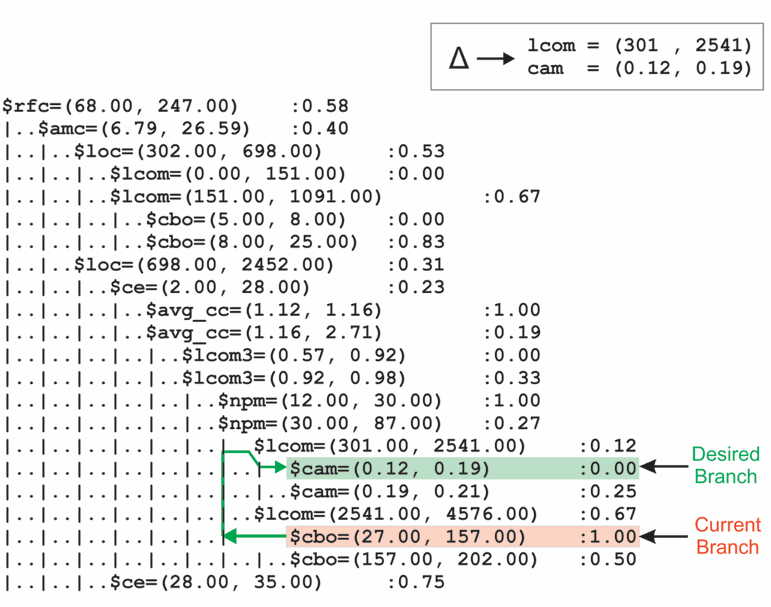
\includegraphics[width=\linewidth]{figs/XTREE_samp.png}
\end{minipage}
~\hrule~
 \caption{A brief tutorial on XTREE.} \label{fig:xtree_samp}
\end{figure*}

\subsubsection{Discussion }\label{sect:disc}
The advantage of the outlier-based
approaches is that they are simple to implement, but the approaches have   two  major disadvantages. 
First, they are {\em verbose}. A threshold can be calculated for every metric -- so, which one should the developers focus on changing? Without a means for prioritizing the  thresholds and metrics against one another, developers may have numerous or conflicting recommendations on what to improve. Second, the outlier approaches suffers from
the {\em disjunction} problem.
That is, while
 they propose thresholds for many code metrics
individually, they make no comment on what
metrics need to be changed at the same time. 



\subsection{Cluster Deltas}

Cluster deltas are a general method
for learning {\em conjunctions} of changes
that need to be applied at the same time. 
This approach works as follows:
\begin{itemize}
    \item Cluster the data. 
    \item Find
neighboring clusters $C_+,C_-$ where $C_+$ has more examples of defective
modules than $C_-$;
\item Compute the  delta   in code metrics between the clusters using \mbox{$\Delta = C_+ - C_-$}, i.e.
{\em towards} the cluster with lower defects;
\item $\Delta$ are changes needed in defective modules of $C_+$ to
      make them more like the less-defective modules of $C_-$
\end{itemize}
Note that $\Delta$ is a conjunction of  recommendations.
Since it is computed
from neighboring clusters, the examples contain similar distributions and $\Delta$ respects the naturally occurring constraints in the data. For example,
given a bad smell pertaining to large methods,   $\Delta$   will not  suggest lowering lines of code
without also increasing a coupling measure. 
Cluster deltas are used in CD~\cite{me12c} and XTREE.

\subsubsection{CD}
Borges and Menzies first proposed the CD centroid delta approach to
generate {\em conjunctions} of code metrics
that need to be changes at the same time
in order to reduce defects~\cite{me12c}.
CD used the WHERE clustering algorithm developed by the
authors for a prior application~\cite{localvsglobal}.
Each cluster was then replaced by its centroid
and $\Delta$ was calculated directly from the difference
between code metrics values between one centroid
and its nearest neighbor.


As shown below, one drawback with with CD is that it is {\em verbose}
since
CD   recommended changes to all code
metrics with different values in those two centroids. 
This makes it hard to use CD to   critique and prune away bad smells. Further, CD will be shown to be
not as effective
in proposing changes to reduce defects as XTREE.

\subsubsection{XTREE: Overview}

  XTREE  is a cluster delta algorithm
  that avoids the problem of verbose $\Delta$s.
  Instead of reasoning over cluster centroids,
  XTREE utilizes a decision tree learning approach
  to find the fewest differences between clusters of examples.
  
  
 XTREE uses an iterative dichotomizer that
first converts the values for each code
metrics into a small number of ranges.
Consider a code metric is split into $r$ ranges and each range is of
  size
    $n_r$ is
  associated with a set of defect counts $x$ with standard deviation
  $\sigma_r$.
  The best split for that range is
  the one that minimizes the expected value of the
  defect variance, after the split; i.e.
  $\sum_r\frac{n_r}{n}\sigma_x$ (where $n=\sum_r n_r$).
  This discretizer then recurses on each part of the split
  to find other splits. 
  
  When discretization finishes, each code metric $M$ has a 
  final expected value $M_v$ for the defect standard deviation 
  across all the discretized ranges of that metric.
  Iterative dichomization sorts the metrics by $M_c$
  to find the best ``splitter'' for the data
  (the code metric with smallest $M_v$). The data
  is then split on the ranges of the splitter and
  iterative dichomization recurses on each range.  In this way,
  each split is the root of a sub-tree.
  

 
  While not usually labelled as such, iterative dichomization can
  be viewed as a clustering algorithm that groups together code modules
  with similar defect counts and some shared ranges of code metrics.
  For our purposes, we score each cluster found in this way according
  to the percent of classes with known defects. For example,
  the last line of \fig{xtree_samp} shows a tree lead with 75\%
  defective modules.
  
 \fig{xtree_samp} offers
  a small example of how XTREE builds
    $\Delta$ by comparing branches that lead to leaf clusters
  with different defect percentages. In this example, assume a project with a table of code metrics data describing its classes in the form of \fig{ck}. After code inspections and running test cases or operational
      tests, each such class is augmented with a defect count.
      Iterative dichomization takes that table of data and, 
        generates the tree of \fig{xtree_samp}.
        
     Once the tree is built, a class with code metric data is passed into the tree and evaluated down the tree to a leaf node (see the \textcolor{orange}{{\bf orange}} line in \fig{xtree_samp}).
      XTREE then looks for a nearby leaf node with a lower defect
      count (see the \textcolor{green}{{\bf green}} line in \fig{xtree_samp}). For that evaluated class, XTREE proposes a bad smell
      thresholds that is  the difference between 
      \textcolor{green}{{\bf green}} and \textcolor{orange}{{\bf orange}}. 
  
  
\subsubsection{XTREE:   Details}

Using the training data,  XTREE uses  
iterative dichomization to
  divide  $N$ code modules  into  clusters of
size $\sqrt{N}$.

Next, for each test code module, 
	  find $C_+$ as follows take each test , run it down to a leaf in the decision tree.  
After that,	  find $C_-$ as follows:
		\begin{itemize}
		\item Starting at the  $C_+$ leaf, ascend   $lvl\in \{0,1,2...\}$ tree levels;
		\item Identify {\em sibling} leaves; i.e. leaf clusters that can be reached from level $lvl$ that are not same as {\em current }
		\item Find the {\em better} siblings; i.e. those 50\% (or less)
		fewer defects than $C_+$.
		   If none found, then repeat for $lvl += 1$. Also,
		    return nil  if the new $lvl$ is above the root. 
		\item  Set $C_-$ to the  {\em closest} better sibling where distance is measured between the mean centroids of that sibling and {\em current}
		\ei
	 Now find $\Delta = C_+ - C_-$  by reflecting
	 on the set difference between  conditions in the decision tree branch to $C_-$ and $C_+$. To find that delta,
	 for discrete attributes, the delta is the value from {\em desired};
	    for numerics  expressed as ranges, the delta is a random number selected from the low and high boundaries of the that range. 
	  

\begin{figure*}[!t]
	\small
	\begin{center}
		\begin{minipage}{.46\linewidth}
			\begin{tabular}{r@{~}|l@{~}|r@{~}|l@{~}|r@{~}|r@{~}|} \cline{2-6}
			 
				
				& \multicolumn{5}{c|}{ Data set  properties}\\ 
			 
				& \multicolumn{2}{c|}{training}   & \multicolumn{3}{c|}{testing}      \\ \cline{2-6}
				data set      & versions           & cases & versions     & cases    & \% defective             \\ \hline
				jedit    & 3.2, 4.0, 4.1, 4.2 & 1257      & 4.3          & 492          & 2 \\
				ivy      & 1.1, 1.4           & 352       & 2.0          & 352          & 11 \\
				camel    & 1.0, 1.2, 1.4      & 1819      & 1.6          & 965          & 19 \\
				ant      & 1.3, 1.4, 1.5, 1.6 & 947       & 1.7          & 745          & 22 \\
				synapse  & 1.0, 1.1           & 379       & 1.2          & 256          & 34 \\
				velocity & 1.4, 1.5           & 410       & 1.6          & 229          & 34 \\
				lucene   & 2.0, 2.2           & 442       & 2.4          & 340          & 59 \\
				poi      & 1.5, 2, 2.5        & 936       & 3.0          & 442          & 64 \\
			 xerces   & 1.0, 1.2, 1.3      & 1055      & 1.4          & 588          & 74  \\ 
			 log4j    & 1.0, 1.1           & 244       & 1.2          & 205          & 92   \\
			 xalan    & 2.4, 2.5, 2.6      & 2411      & 2.7          & 909          & 99  \\\hline 
				
				
			\end{tabular}\end{minipage}~~~~~~\begin{minipage}{.4\linewidth}
			\begin{tabular}{|rrr|rrr|rr|l} \cline{1-8}
			 
				\multicolumn{8}{|c|}{  Results from learning}\\
			 
				\multicolumn{3}{|c|}{untuned} & \multicolumn{3}{c|}{tuned} & \multicolumn{2}{c|}{change}\\
				\cline{1-8}
				
				pd & pf & good? & pd & pf & good? & pd & pf\\\cline{1-8}
				\rowcolor{celadon}55 & 29 &   & 64 & 29 & y & 9 & 0&$\star$\\
				\rowcolor{celadon}	65 & 35 & y & 65 & 28 & y & 0 & -7&$\star$\\
				49 & 31 &   & 56 & 37 &   & 5 & 6\\
				\rowcolor{celadon}	49 & 13 & y & 63 & 16 & y & 14 & 3&$\star$\\
				45 & 19 &   & 47 & 15 &   & 2 & -4\\
				78 & 60 &   & 76 & 60 &   & -2 & 0\\
				56 & 25 &   & 60 & 25 & y & 4 & 0\\
				\rowcolor{celadon}	56 & 31 &   & 60 & 10 & y & 4 & -21&$\star$\\
			\rowcolor{lavenderpink}	30 & 31 &   & 40 & 29 &   & 10 & -2&$\times$\\
				\rowcolor{lavenderpink}32 & 6 &   & 30 & 6 &   & -2 & 0&$\times$\\
				\rowcolor{lavenderpink}38 & 9 &   & 47 & 9 &   & 9 & 0&$\times$\\
				\hline 
			\end{tabular}
			
		\end{minipage}
	\end{center}    
	
	\caption{Training and test {\em data set properties} for  Jureczko data ,
		sorted by \% defective examples.
		On the right-hand-side, we show the {\em results from learning}.
		Data is usable if it has a recall of 60\% or more and false alarm of 30\% or less (and note that, after tuning, there are more usable data sets than before). Results  	\colorbox{celadon}{ marked with ``$\star$''} show large improvements in performance, after tuning
		(lower {\em pf} or higher {\em pd}).
		Data in  the  \colorbox{lavenderpink}{three bottom rows}, marked with ``$\times$'', are  performing
		poorly-- that data so many defective examples  that it  is hard for
		our learners to distinguish between classes.
	}\label{fig:j}
\end{figure*}
      
\section{Evaluation}
\subsection{Research Questions}
% To define our experiments, we  review some details
% about XTREE. 

 XTREE proposes
conjunctions of changes that might perform better than
the disjunctions proposed by Shatnawi and Alves et al.
Unlike CD, XTREE should be less verbose since
it only reports the deltas in the code
metrics rather than values for all metrics.
To evaluate XTREE,
we propose four research questions.

\subsubsection{ RQ1: Effectiveness} \label{sect:rq}

{\em In a comparison of   outlier and cluster delta
methods, which one most reduces the expected number
of defects?}

To find an answer to this question, we will assume that developers
refactor their code until the bad smell thresholds is not violated.
This refactoring will start with some {\em initial} code
base that is changed to a {\em new} code base. 
For example, if the bad smell is \mbox{{\em loc $>100$}} and a 
code module has 500 lines of code, we reason
optimistically that we can change that code metric
to 100.  
Using a defect
predictor learned via Random Forest, we then predict the
number of defects in $d_+,d_-$ in {\em initial} and {\em new}. We evaluate the performance of XTREE, CD, Shatnawi, and Alves methods in setting bad smell thresholds.
The best bad smell threshold method is the one that maximizes
\begin{equation}\label{eq:diff}
\mathit{improvement} = 100* \left(1 - \frac{ d_- }{ d_+}\right)
\end{equation}

\subsubsection{RQ2: Verbosity} 

{\em In a comparison of    outlier and cluster delta
methods, which one proposes the fewest thresholds?}

Note that this is important since our goal is to critique and, possibly,
reject irrelevant bad smell detectors. As mentioned above,
  verbosity makes it hard   to critique and prune bad smells
since any bad smell mentioned by a developer has some support
somewhere amongst all those proposed thresholds. 

To measure verbosity, we will compare the counts of how often
different approaches assign thresholds to code metrics
(and the one that makes the least assignments is the least verbose).

\subsubsection{RQ3: Optimality}  

{\em How consistent are the leaves of XTREE?}

Before using XTREE to critique bad smell detectors, it is important to analyze the quality XTREE. Such analysis allows users to determine the credibility of the critiques offered. 

To measure the optimality we measure the discriminatory power of the tree as suggested by ~\cite{osei04}. (Note: this is done in addition to the most commonly used performance criterion (i.e.
correct classification rate). For XTREE (with binary target variables) we present the probability of false alarm (PF) and the probability of detection (pf) in \fig{j}.)


\subsubsection{RQ4: Understanding Co-changes} 

{\em In a comparison of outlier and cluster delta
methods, which one is aware of the existing associations between software metrics?}

Our goal is to critique and, possibly, reject irrelevant bad smell detectors. However, with low verbosity there exists the risk of ignoring underlying associations that exist between software metrics. Failure to respect this challenges the validity of the critiques. 


To measure if our methods respect these co-changes in metrics, we will compare the medians of each of the metrics. Statistically significant changes in all co-varying metrics will indicate our method's efficacy in respecting these underlying associations.
 
 
\subsection{Test Data}\label{sect:tesd}

To explore these research questions,
we used data from
Jureczko et al.'s collection of object-oriented Java systems~\cite{jureczko10}. To access that data, go to   git.io/vGYxc.
The Jureczko data records the number of known defects for each class using a post-release bug tracking system. The classes are described in terms of nearly two dozen metrics included in the Chidamber and Kemerer metric suite, such as number of children (noc), lines of code (loc), etc. For details on the Jureczko code
metrics, see  \fig{ck}. For details on the rows and versions
of that data, see the left-hand-side columns of \fig{j}.



 
\subsection{Assessment Oracles}
\label{sect:eval}
We must be able to assess how defective the code is before and after a proposed refactoring. Since we do not have actual  examples of defect counts post-refactoring, we   approximate   defect counts after the   changes   (as changes to the code metrics).

Prior work~\cite{Cheng10,OKeeffe08,OKeeffe07,Moghadam2011,Mkaouer14} 
used the QMOOD   quality model ~\cite{Bansiya02} to assess the results of their refactorings
Since the QMOOD method based on old (2002) project data, we use Random Forests~\cite{Breiman2001} to build
the assessment methods.
  Random Forests are a decision tree learning method but
  instead of building one tree, hundreds are built using
  randomly selected subsets of the data. The final predictions
  come from averaging the predictions over all the trees.
  Recent studies endorsed the use
  of  Random Forests for  defect prediction~\cite{lessmann}.
  
\fig{j} shows   studies with Random Forests and
the Jureczko data. Given   $V$ released versions, we test on version $V$ and train on the available data from $V-1$ earlier releases (as shown in \fig{j}. Note the   \colorbox{lavenderpink}{three bottom rows}   marked with $\times$: these contain predominately defective classes (two-thirds, or more).  In such data, it is hard to distinguish good examples (due to all the bad examples). 

In order to identify the presence (or absence) of defects, we can   use Boolean classes in the  Jureczko data ( \texttt{True} if defects \textgreater 0; \texttt{False} if defects = 0). For such data, the quality of the predictor can be measured using (1) the  probability of detection (a.k.a. ``pd'' or recall):  the percent of faulty classes in the test data detected by the {\em predictor}; and (2) the  probability of false alarm (a.k.a. ``pf''): the percent of non-fault classes that are {\em predicted} to be defective.

The ``untuned'' columns of \fig{j}
show a preliminary study. This study used
Random Forest with its ``off-the-shelf'' tunings (i.e.  
100 trees per forest).  
The forests were built from training data and applied to test data
not seen during training.  In this
study, we called a data set ``usable'' if   Random Forest was able to classify the instances with a performance threshold of $\mathit{pd}\ge 60 \wedge \mathit{pf} \le 30$\% (determined from standard results in other publications~\cite{me07b}). Note that no  data set meet
that criteria.

The ``tuned'' columns of \fig{j} show that we can salvage some of the data sets. We applied both the SMOTE algorithm and differential evolution to improve the performance of the classifier. Pelayo and Dick~\cite{pelayo07} report that defect prediction is improved by SMOTE~\cite{Chawla2002}; i.e. an over-sampling of minority-class examples and an under-sampling of majority-class examples. Fu et al.~\cite{fu:ase15} report that parameter tuning with differential evolution~\cite{storn97} can quickly explore the tuning options of Random Forest to find better settings for the (e.g.) size of the forest, the termination criteria
for tree generation, etc. We note that SMOTE-ing and
parameter tunings were applied to the training data only and not to the test data.

The rows \colorbox{celadon}{marked with a $\star$} in \fig{j} show data sets whose performance was improved remarkably by these techniques. For example, in {\em poi}, the recall increased by 4\% while the false alarm rate dropped by 21\%. However, as might have been expected, we could not salvage the data sets in the  three bottom rows.

We eliminate the data sets for which we could not build an adequately performing Random Forest classifier with $\mathit{pd}\ge 60 \wedge \mathit{pf} \le 30$\%. Thus, our analysis uses the {\em jedit, ivy, ant, lucene} and {\em poi} for evaluating recommended changes.




\subsection{Statistics}


We use 40 repeated runs, each with different random number seeds (we use 40 since that is  more than the 30 samples  needed to satisfy the central limit theorem). Each run collects the \eq{diff} values.
We use multiple runs since two of our methods use some random choices: CD uses the  stochastic WHERE clustering algorithm~\cite{localvsglobal}
while XTREE non-deterministically picks thresholds randomly from
the high and low boundary of a range. 
 Hence, to compare all
four methods, we must run the analysis many times. 



\begin{figure}[!htbp]
%{\scriptsize \textbf{Ant}\\[0.1cm]}


{\scriptsize \hspace{3.5cm}\underline{Observed Improvements (from \eq{diff})}}\vspace{2mm}
 

{\scriptsize \textbf{Ant}~~~~~~~~ \begin{tabular}{{l@{~~~~}l@{~~~~}|r@{~~~~}r@{}c@{~~~}r}}
\arrayrulecolor{lightgray}
\rowcolor{lightgray}\textbf{Rank} & \textbf{Treatment} & \textbf{Median} & \textbf{IQR~~~} & \\
  1 &         XTREE &    56   &  21  & \quart{54}{25}{65}{1} \\
\hline  2 &        Alves &    32   &  17  & \quart{28}{20}{37}{1} \\
\hline  3 &     Shatnawi &    15   &  4.2 & \quart{15}{6}{18}{1} \\
  3 &           CD &    12   &  0  & \quart{15}{0}{15}{6} \\
\hline \end{tabular}}\\

%{\scriptsize \textbf{Lucene}\\[0.1cm]}
%{\scriptsize \textbf{Poi}\\[0.1cm]}
{\scriptsize 

\textbf{Poi}~~~~~~~~ \begin{tabular}{{l@{~~~~}l@{~~~~}|r@{~~~~}r@{~~}c@{}r}}
\arrayrulecolor{lightgray}
\rowcolor{lightgray}\textbf{Rank} & \textbf{Treatment} & \textbf{Median} & \textbf{IQR~~~} & \\
        1 &         XTREE &    20   &  16  & \quart{39}{40}{51}{2} \\
\hline  2 &        Alves &    14   &  16  & \quart{21}{41}{37}{2} \\
\hline  3 &           CD &    11   &  0  & \quart{23}{0}{23}{7} \\
        3 &     Shatnawi &    8   &  1  & \quart{19}{5}{21}{2} \\
\hline \end{tabular}}\\

{\scriptsize \textbf{Lucene}~ \begin{tabular}{{l@{~~~~}l@{~~~~}|r@{~~~~}r@{~~}c@{}r}}
\arrayrulecolor{lightgray}
\rowcolor{lightgray}\textbf{Rank} & \textbf{Treatment} & \textbf{Median} & \textbf{IQR~~~} & \\
        1 &         XTREE &    16   &  6  & \quart{50}{29}{71}{4} \\
        1 &     Shatnawi  &    15   &  2  & \quart{63}{10}{67}{4} \\
\hline  2 &           CD  &    13   &  0  & \quart{55}{0}{55}{6} \\
\hline  3 &        Alves  &    9   &  4  & \quart{33}{19}{42}{4} \\
\hline \end{tabular}}\\


%{\scriptsize \textbf{Ivy}\\[0.1cm]}
{\scriptsize \textbf{Ivy}~~~~~~~~ \begin{tabular}{{l@{~~~~}l@{~~~~}|r@{~~~~}r@{~~}c@{}r}}
\arrayrulecolor{lightgray}
\rowcolor{lightgray}\textbf{Rank} & \textbf{Treatment} & \textbf{Median} & \textbf{IQR~~~} & \\
        1 &        Alves &    67   &  20  & \quart{58}{21}{71}{1} \\
\hline  2 &         XTREE &    52   &  22  & \quart{42}{24}{55}{1} \\
\hline  3 &           CD &    35   &  0  & \quart{27}{0}{27}{2} \\
\hline  4 &     Shatnawi &    20   &  7  & \quart{18}{8}{21}{1} \\
\hline \end{tabular}}\\

%{\scriptsize \textbf{Jedit}\\[0.1cm]}

{\scriptsize  \textbf{Jedit}~~~~~~~ \begin{tabular}{{l@{~~~}l@{~~~~}|r@{~~~~}r@{~~}c@{}r}}
\arrayrulecolor{lightgray}
\rowcolor{lightgray}\textbf{Rank} & \textbf{Treatment} & \textbf{Median} & \textbf{IQR~~~} & \\
  1 &        Alves &    36   &  7  & \quart{60}{10}{66}{1} \\
  1 &        XTREE &    36   &  0  & \quart{66}{0}{66}{2} \\
  1 &     Shatnawi &    36   &  9  & \quart{53}{13}{66}{1} \\
  1 &          CD &    36   &  0  & \quart{66}{0}{66}{2} \\
\hline \end{tabular}}\\
\caption{Results for {\bf RQ1} from the
Jureczko   data sets.  Results from 40 repeats.
Values come from \eq{diff}.
Values near 0
imply no improvement,
{\em Larger} median values are {\em better}. 
Note that XTREE and Alves are usually best and CD and Shatnami
are usually worse.}
\label{fig:jur}
\end{figure}

% ## ant

% {\scriptsize \begin{tabular}{l@{~~~}l@{~~~}r@{~~~}r@{~~~}c}
% \arrayrulecolor{lightgray}
% \textbf{XTREE} & \textbf{Treatment} & \textbf{Median} & \textbf{IQR} & \\\hline
%   1 &     Shatnawi &    15.66  &  4.82 & \quart{15}{6}{18}{1} \\
% \hline  2 &        Alves &    32.53  &  17.47 & \quart{28}{20}{37}{1} \\
% \hline  3 &         XTREE &    56.02  &  21.68 & \quart{54}{25}{65}{1} \\
% \hline \end{tabular}}


% ## ivy

% {\scriptsize \begin{tabular}{l@{~~~}l@{~~~}r@{~~~}r@{~~~}c}
% \arrayrulecolor{lightgray}
% \textbf{XTREE} & \textbf{Treatment} & \textbf{Median} & \textbf{IQR} & \\\hline
%   1 &     Shatnawi &    20.0  &  7.5 & \quart{18}{8}{21}{1} \\
% \hline  2 &         XTREE &    52.5  &  22.5 & \quart{42}{24}{55}{1} \\
% \hline  3 &        Alves &    67.5  &  20.0 & \quart{58}{21}{71}{1} \\
% \hline \end{tabular}}


% ## jedit

% {\scriptsize \begin{tabular}{l@{~~~}l@{~~~}r@{~~~}r@{~~~}c}
% \arrayrulecolor{lightgray}
% \textbf{XTREE} & \textbf{Treatment} & \textbf{Median} & \textbf{IQR} & \\\hline
%   1 &     Shatnawi &    36.36  &  9.09 & \quart{53}{13}{53}{1} \\
%   1 &         XTREE &    36.36  &  0.0 & \quart{53}{0}{53}{1} \\
%   1 &        Alves &    45.45  &  27.28 & \quart{39}{40}{66}{1} \\
% \hline \end{tabular}}


% ## lucene

% {\scriptsize \begin{tabular}{l@{~~~}l@{~~~}r@{~~~}r@{~~~}c}
% \arrayrulecolor{lightgray}
% \textbf{XTREE} & \textbf{Treatment} & \textbf{Median} & \textbf{IQR} & \\\hline
%   1 &        Alves &    9.85  &  4.44 & \quart{33}{19}{42}{4} \\
% \hline  2 &     Shatnawi &    15.76  &  2.45 & \quart{63}{10}{67}{4} \\
%   2 &         XTREE &    16.75  &  6.9 & \quart{50}{29}{71}{4} \\
% \hline \end{tabular}}


% ## poi

% {\scriptsize \begin{tabular}{l@{~~~}l@{~~~}r@{~~~}r@{~~~}c}
% \arrayrulecolor{lightgray}
% \textbf{XTREE} & \textbf{Treatment} & \textbf{Median} & \textbf{IQR} & \\\hline
%   1 &     Shatnawi &    8.53  &  1.78 & \quart{19}{5}{21}{2} \\
% \hline  2 &        Alves &    14.95  &  16.38 & \quart{21}{41}{37}{2} \\
% \hline  3 &         XTREE &    20.64  &  16.02 & \quart{39}{40}{51}{2} \\
% \hline \end{tabular}}



To rank these 40 numbers collected from CD, XTREE, Shatnawi, and Alves et al., we use the Scott-Knott test recommended by Mittas and Angelis~\cite{mittas13}. 
Scott-Knott is a top-down clustering approach used to rank different
treatments. If that clustering finds an interesting division of the data, then
some statistical test is applied to the two divisions to check if they
are statistically significant different. If so, Scott-Knott recurses
into both halves.

To  apply Scott-Knott,
  we
sorted a list of  $l=40$ values of \eq{diff} values found in  $ls=4$ different methods. 
Then, we split $l$ into sub-lists $m,n$ in order to maximize the expected value of differences in the observed performances before and after divisions. E.g. for lists $l,m,n$ of size $ls,ms,ns$ where $l=m\cup n$: \[E(\Delta)=\frac{ms}{ls}abs(m.\mu - l.\mu)^2 + \frac{ns}{ls}abs(n.\mu - l.\mu)^2\]
We then apply a apply a statistical hypothesis test $H$ to check
if $m,n$ are significantly different  (in our case, the conjunction of A12 and bootstrapping). If so, Scott-Knott recurses on the splits. In other words, we divide the data if \textit{both} bootstrap sampling and effect size test agree that a division is statistically significant (with a confidence of 99\%) and not a small effect ($A12 \ge 0.6$).
For a justification of the use of non-parametric bootstrapping, see Efron \& Tibshirani~\cite[p220-223]{efron93}. For a justification of the use of effect size tests see Shepperd\&MacDonell~\cite{shepperd12a}; Kampenes~\cite{kampenes07}; and Kocaguenli et al.~\cite{Kocaguneli2013:ep}. These researchers warn that even if a hypothesis test declares two populations to be ``significantly'' different, then that result is misleading if the ``effect size'' is very small. Hence, to assess the performance differences we first must rule out small effects using A12, a test   recently endorsed by Arcuri and Briand at ICSE'11~\cite{arcuri11}.

The Scott-Knott  results are presented in the form of line diagrams like those shown on the right-hand-side of \fig{jur}.
The black dot shows the median \eq{diff} values and the horizontal lines stretch 
from the 25th percentile to the 75th percentile (the inter-quartile range, IQR).
As an example of how to read this table, consider the {\em Ant}
results. Those rows are  sorted on the median values of each method. Note that all the methods have \eq{diff} \textgreater $ 0\%$; i.e. all these methods reduced the expected value of the performance score in that experiment while XTREE achieved the greatest reduction (of 56\% from the original value).
These results table has a  left-hand-side  {\bf Rank} column, computed using the
Scott-Knott test described above. In the {\em Ant}
results, XTREE is ranked the best, while CD is  ranked   worst.

% Please add the following required packages to your document preamble:
% \usepackage{multirow}
% \usepackage[table,xcdraw]{xcolor}
% If you use beamer only pass "xcolor=table" option, i.e. \documentclass[xcolor=table]{beamer}
\newcommand{\ZZ}{.}
\begin{figure*}
\renewcommand{\baselinestretch}{0.8} 
\scriptsize  
\centering

\label{my-label}
                  
\begin{tabular}{c|rrrr|rrrr|rrrr|rrrr|rrrr}
\multicolumn{1}{c}{\cellcolor[HTML]{EFEFEF}{\color[HTML]{000000} }} & \multicolumn{4}{c}{\cellcolor[HTML]{EFEFEF}{\color[HTML]{000000} Ant}} & \multicolumn{4}{c}{\cellcolor[HTML]{EFEFEF}{\color[HTML]{000000} Ivy}} & \multicolumn{4}{c}{\cellcolor[HTML]{EFEFEF}{\color[HTML]{000000} Lucene}} & \multicolumn{4}{c}{\cellcolor[HTML]{EFEFEF}{\color[HTML]{000000} Jedit}} & \multicolumn{4}{c}{\cellcolor[HTML]{EFEFEF}{\color[HTML]{000000} Poi}} \\
\multicolumn{1}{c@{}}{\multirow{-2}{*}{\cellcolor[HTML]{EFEFEF}{\color[HTML]{000000} Features}}} & \multicolumn{1}{c@{}}{\cellcolor[HTML]{EFEFEF}{\color[HTML]{000000} XTREE}} & \multicolumn{1}{c@{}}{\cellcolor[HTML]{EFEFEF}{\color[HTML]{000000} CD}} & \multicolumn{1}{c@{}}{\cellcolor[HTML]{EFEFEF}{\color[HTML]{000000} Alves}} & \multicolumn{1}{c@{}}{\cellcolor[HTML]{EFEFEF}{\color[HTML]{000000} Shatn}} & \multicolumn{1}{c@{}}{\cellcolor[HTML]{EFEFEF}{\color[HTML]{000000} XTREE}} & \multicolumn{1}{c@{}}{\cellcolor[HTML]{EFEFEF}{\color[HTML]{000000} CD}} & \multicolumn{1}{c@{}}{\cellcolor[HTML]{EFEFEF}{\color[HTML]{000000} Alves}} & \multicolumn{1}{c@{}}{\cellcolor[HTML]{EFEFEF}{\color[HTML]{000000} Shatn}} & \multicolumn{1}{c@{}}{\cellcolor[HTML]{EFEFEF}{\color[HTML]{000000} XTREE}} & \multicolumn{1}{c@{}}{\cellcolor[HTML]{EFEFEF}{\color[HTML]{000000} CD}} & \multicolumn{1}{c@{}}{\cellcolor[HTML]{EFEFEF}{\color[HTML]{000000} Alves}} & \multicolumn{1}{c@{}}{\cellcolor[HTML]{EFEFEF}{\color[HTML]{000000} Shatn}} & \multicolumn{1}{c@{}}{\cellcolor[HTML]{EFEFEF}{\color[HTML]{000000} XTREE}} & \multicolumn{1}{c@{}}{\cellcolor[HTML]{EFEFEF}{\color[HTML]{000000} CD}} & \multicolumn{1}{c@{}}{\cellcolor[HTML]{EFEFEF}{\color[HTML]{000000} Alves}} & \multicolumn{1}{c@{}}{\cellcolor[HTML]{EFEFEF}{\color[HTML]{000000} Shatn}} & \multicolumn{1}{c@{}}{\cellcolor[HTML]{EFEFEF}{\color[HTML]{000000} XTREE}} & \multicolumn{1}{c@{}}{\cellcolor[HTML]{EFEFEF}{\color[HTML]{000000} CD}} & \multicolumn{1}{c@{}}{\cellcolor[HTML]{EFEFEF}{\color[HTML]{000000} Alves}} & \multicolumn{1}{c@{}}{\cellcolor[HTML]{EFEFEF}{\color[HTML]{000000} Shatn}} \\
wmc & \ZZ & 92 & 100 & 100 & 18 & 95 & 100 & 100 & 89 & 95 & 100 & \ZZ &\ZZ& 63 & \ZZ &\ZZ& \ZZ & 100 & 100 &\ZZ\\
dit & \ZZ & 77 & 100 & \ZZ & \ZZ & 87 & 100 & \ZZ & \ZZ & 80 & 100 & \ZZ &\ZZ& 72 & 100 & 100 & \ZZ & 46 & 100 &\ZZ\\
noc & \ZZ & 20 & 100 & \ZZ & \ZZ & \ZZ & 100 & \ZZ & \ZZ & 26 & \ZZ &\ZZ& \ZZ &\ZZ& \ZZ &\ZZ& \ZZ &\ZZ& \ZZ &\ZZ\\
cbo & 88 & 99 & 100 & 100 & 91 & 100 & 100 & 100 & 60 & 94 & 100 & 100 & \ZZ & 100 & 100 & \ZZ & 1 & 74 & 100 &\ZZ\\
rfc & 100 & 100 & 100 & \ZZ & 8 & 95 & 100 & \ZZ & 10 & 83 & 100 & \ZZ & 100 & 100 & 100 & 100 & 100 & 95 & 100 &\ZZ\\
lcom & \ZZ & 98 & 100 & 100 & 15 & 100 & 100 & 100 & \ZZ & 94 & 100 & \ZZ &\ZZ& 100 & 100 & \ZZ &\ZZ& 100 & 100 & 100 \\
ca & \ZZ & 93 & 100 & \ZZ & 7 & 95 & 100 & \ZZ & 40 & 89 & 100 & \ZZ &\ZZ& 63 & 100 & 100 & \ZZ & 74 & 100 &\ZZ\\
ce & 5 & 100 & 100 & \ZZ & \ZZ & 97 & 100 & \ZZ &\ZZ& 90 & 100 & \ZZ &\ZZ& 100 & 100 & 100 & \ZZ & 64 & 100 &\ZZ\\
npm & \ZZ & 88 & 100 & \ZZ & 8 & 97 & 100 & \ZZ &\ZZ& 93 & 100 & 100 & \ZZ & 100 & 100 & \ZZ &\ZZ& 100 & 100 &\ZZ\\
lcom3 & \ZZ & 90 & 100 & \ZZ & 7 & 95 & 100 & \ZZ & 13 & 79 & 100 & 100 & \ZZ & 63 & 100 & 100 & \ZZ & 92 & 100 & 100 \\
loc & 100 & 99 & 100 & 100 & 97 & 97 & 100 & 100 & 60 & 100 & 100 & 100 & \ZZ & 100 & \ZZ & 100 & 100 & 100 & 100 & 100 \\
dam & \ZZ & 21 & 100 & \ZZ & \ZZ & 22 & 100 & \ZZ &\ZZ& 55 & 100 & \ZZ &\ZZ& 45 & 100 & 100 & \ZZ & 73 & 100 &\ZZ\\
moa & \ZZ & 67 & 100 & \ZZ & \ZZ & 82 & 100 & \ZZ &\ZZ& 60 & 100 & 100 & \ZZ & 54 & 100 & 100 & \ZZ & 58 & 100 &\ZZ\\
mfa & 5 & 93 & 100 & \ZZ & \ZZ & 90 & 100 & \ZZ & 5 & 80 & 100 & \ZZ &\ZZ& 72 & 100 & \ZZ &\ZZ& 72 & 100 &\ZZ\\
cam & \ZZ & 99 & 100 & 100 & 84 & 100 & 100 & 100 & 10 & 94 & 100 & \ZZ &\ZZ& 100 & 100 & \ZZ &\ZZ& 98 & 100 & 100 \\
ic & \ZZ & 52 & 100 & 100 & \ZZ & 70 & \ZZ &\ZZ& \ZZ & 68 & 100 & \ZZ &\ZZ& 36 & 100 & \ZZ &\ZZ& 43 & 100 & 100 \\
cbm & \ZZ & 59 & 100 & \ZZ & \ZZ & 85 & \ZZ &\ZZ& \ZZ & 71 & 100 & \ZZ &\ZZ& 36 & 100 & 100 & \ZZ & 67 & 100 &\ZZ\\
amc & \ZZ & 99 & \ZZ & \ZZ & \ZZ & 95 & 100 & \ZZ & 30 & 100 & \ZZ & \ZZ & \ZZ & 100 & 100 & 100 & \ZZ & 97 & \ZZ &\ZZ\\
max cc & \ZZ & 87 & 100 & 100 & \ZZ & 85 & 100 & 100 & \ZZ & 71 & \ZZ &\ZZ& \ZZ & 45 & 100 & \ZZ &\ZZ& 63 & 100 &\ZZ\\
avg cc & 12 & 99 & 100 & 100 & \ZZ & 95 & 100 & 100 & 13 & 98 & \ZZ &\ZZ& \ZZ & 100 & 100 & 100 & \ZZ & 92 & 100 & \ZZ\\\hline
\end{tabular}
\caption{Results for {\bf RQ2}.
Percentage counts of  how often an approach recommends changing a code metric
(in 40 runs). ``100'' means that this code metrics
was always recommended. Cells marked with ``.'' indicate  0\%. For the Shatnami and Alves et al.
columns,  metrics score 0\% if they always fail the $p \le 0.05$ test of \tion{p}.
For CD, cells are blank when two centroids have the same value for the same code
metrics. For XTREE, cells are blanks when they do not appear in the delta
between branches.  Note
that XTREE mentions specific code metrics
far fewer times than other methods.}\label{fig:counts}
\end{figure*}
\subsection{Results}
 
 
\begin{figure*}[!t]
\centering
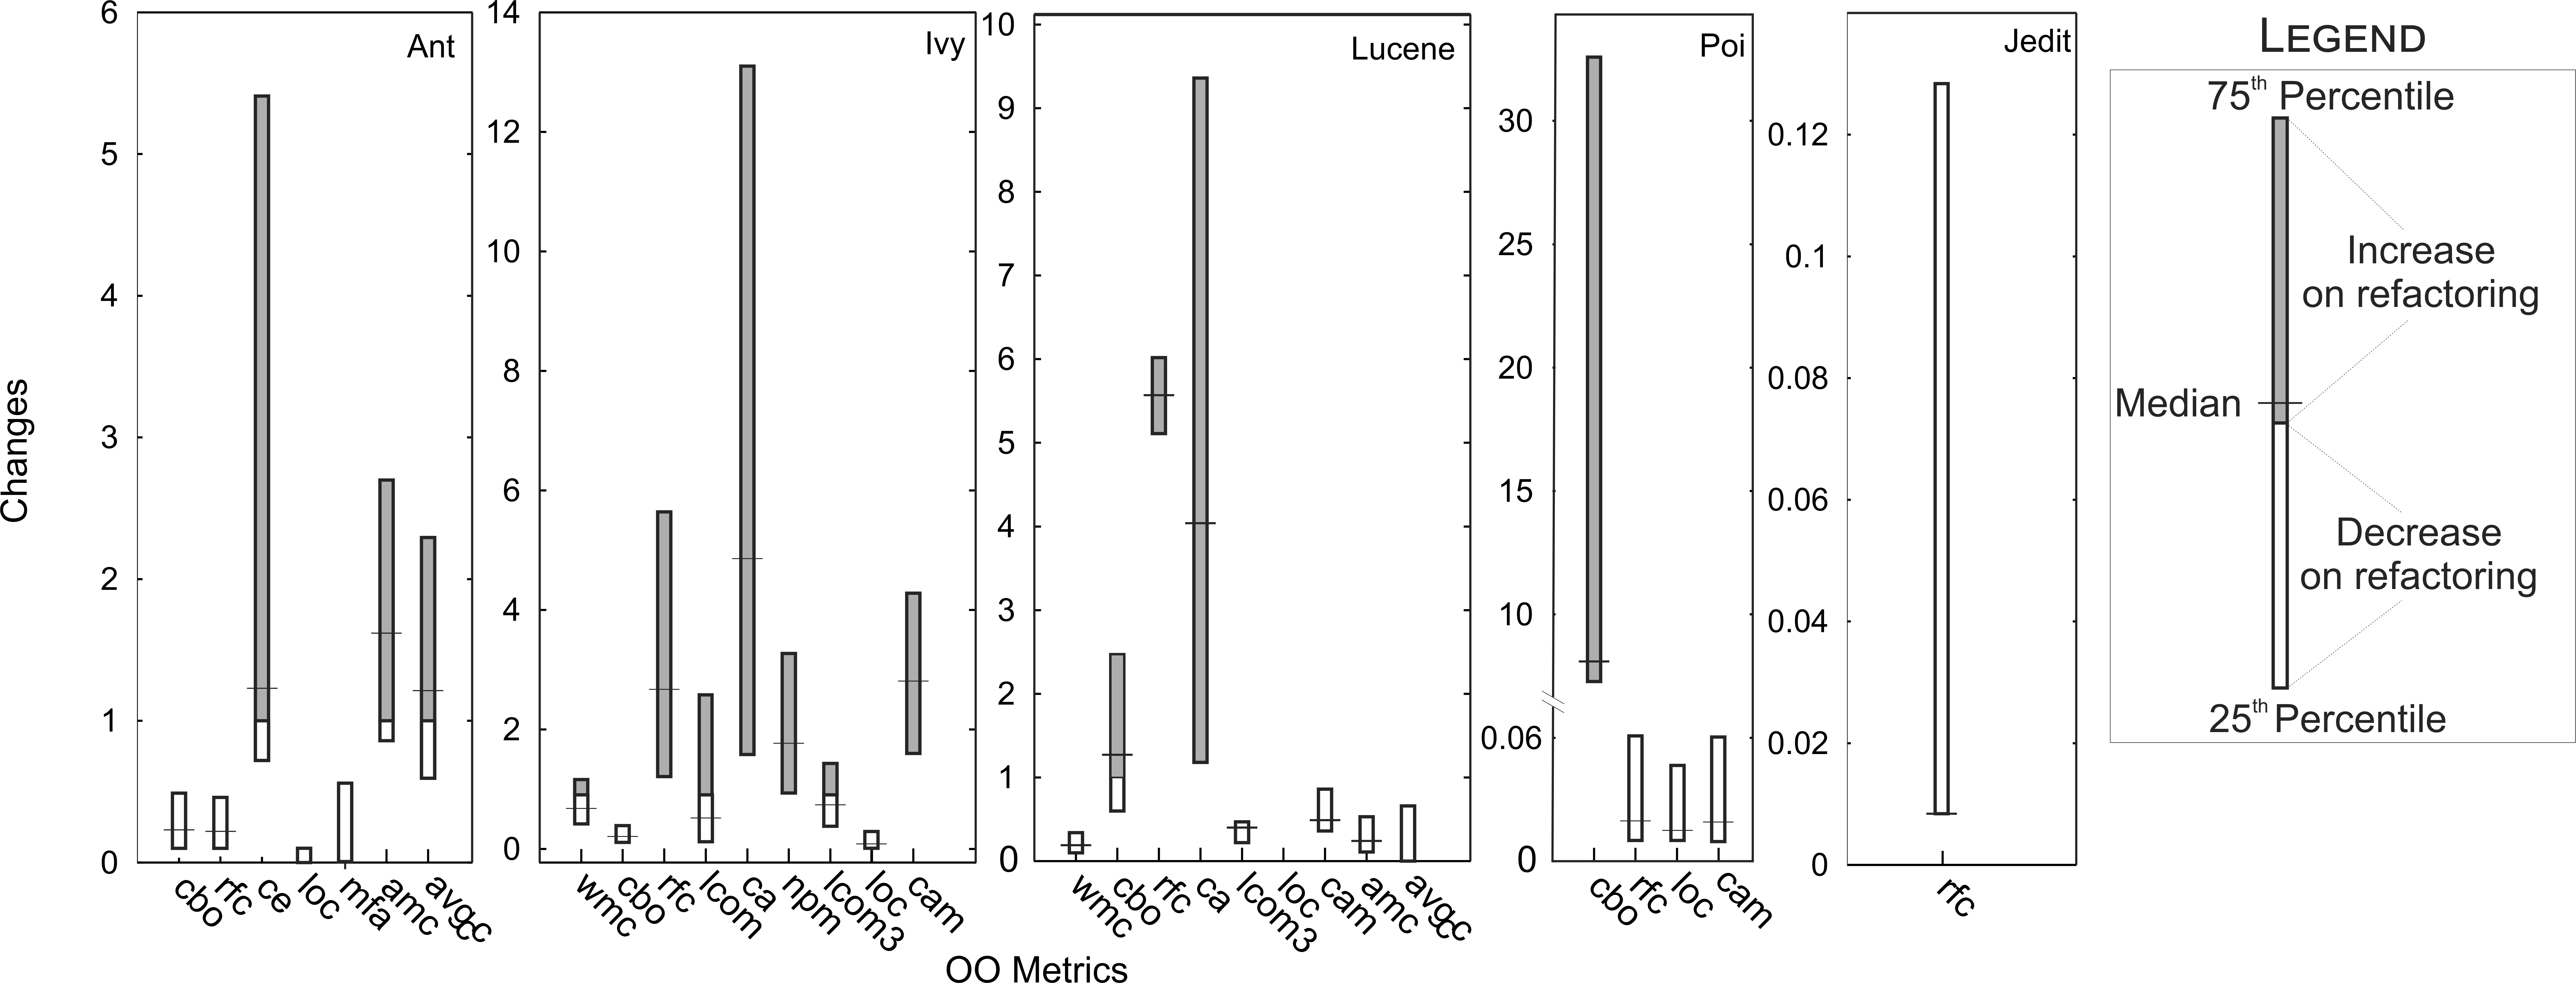
\includegraphics[width=\linewidth]{figs/changes01.png}
\caption{Results  from XTREE.
While \fig{counts} are the {\em number} of times a code metric was changed,
this  figure shows {\em how far} each code metric was changed. Each vertical bar
marks the 27,50,75th percentile change seen in 40 repeats.
All numbers are ratios of initial to final values.
All bar regions marked in gray show {\em increases}.
The interesting feature of these results are that many
of the changes proposed by XTREE require {\em increases}
(this puzzling observation is explained in the text).}
\label{fig:changes}
\end{figure*}



\subsubsection{RQ1: Effectiveness}

\begin{lesson}
In terms of the expected number of defects
  after refactoring,
XTREE is marginally better than Alves. CD and Shatnawi.
on the other hand, usually perform worst.
\end{lesson}
 

{\em In a comparison of   outlier and cluster delta
methods, which one most reduces the expected number
of defects?}

\fig{jur} shows the comparison results.  The Alves and Shatnawi
entries show the net effects of applying (separately) all the disjuncts
proposed by those methods. In this part of the  analysis,
we applied Scott-Knott to all the \eq{diff} values
seen when code metrics were changed
according to the  Alves and Shatnawi


Two data sets are very responsive to defect reduction suggestions:
 Ant, and Ivy (both of which show best case improvements over 50\%).
 The  expected value of defects  
 is changed less in Jedit. This data sets' results
 surprisingly uniform; i.e.   all methods
 find the same ways to reduce the expected number of
defects.   For an explanation of the Jedit uniformity, see \tion{inc}.

Two data sets are not very responsive to defect reduction:
Poi and Lucene. The reason for this can be see in \fig{j}:
both these data sets contain more than 50\% defective modules.
In that space, all our  methods lack a large sample of
defect-free examples. 

Also consider the relative
rank of the different approaches,
 CD and Shatnawi usually  perform comparatively worse while  XTREE gets top ranked position the most
number of times. That said, Alves sometimes beats XTREE (see Ivy)
while sometimes it ties (see Jedit).


Another interesting feature of the XTREE results of
\fig{jur} was that the used code metrics vary
from data set to data set. While changing lines of
code {\em loc} was important in all data sets, 
the other code metrics used were often different.

 
 \subsubsection{RQ2: Verbosity}

{\em In a comparison of outlier and cluster delta methods, which one proposes the fewest thresholds?}

\fig{counts} shows the frequency with which the methods
recommend changes to specific code methods.
Note that XTREE proposes thresholds to
few code metrics compared to the other approaches. 

% COMMENT From LL: This is such a strange way of putting this lesson, and you haven't actually evaluated this.
% 


When combining  \fig{jur} with \fig{counts}, we   see that
even though XTREE proposes changes to far fewer code metrics, those few
code metrics are usually just as effective (or
more effective) than the multiple
thresholds
proposed by CD, Shatnawi or Alves.  That is, XTREE proposes
{\em fewer} and better thresholds than the other approaches studied here.

\begin{lesson}
XTREE finds finds far fewer recommended changes to code metrics, and yet performs as good as or better than other methods in recommending changes that results in fewer defects.
\end{lesson}

% Please add the following required packages to your document preamble:
% \usepackage{graphicx}
\begin{figure*}
\centering
\resizebox{\textwidth}{!}{%
\begin{tabular}{l|c|c|c|c|c|c|c|c|c|c|c|c|c|c|c|c|c|c|c|c}
         & wmc & dit & noc & cbo & rfc & lcom & ca & ce & npm & lcom3 & loc & dam & moa & mfa & cam & ic & cbm & amc & max\_cc & avg\_cc \bigstrut\\ \hline
Ant      &  & & & $-$ &$-$&  & &$+$& & &$-$& & &$-$& & &  &$+$&     &$+$\bigstrut\\ \hline

Ivy      &$-$& & &$-$&$+$&$-$&$+$& &$-$&$-$&$-$& & & &$+$& & & &     &      \bigstrut\\ \hline

Poi      & & & &$+$&$-$& & & & & &$-$& & & &$-$& & & & & \bigstrut\\ \hline

Lucene   &$-$& & &$+$&$+$& &$+$& & &$-$&$-$& & & &$-$& & &$-$& &$-$\bigstrut\\ \hline

Jedit    & & & & &$-$& & & & & & & & & & & & & & &     \bigstrut\\ 

\end{tabular}}

\caption{Direct of changes seen in  
a comparison of statistically significantly different static code attributes measures seen in the clusters found by XTREE. Each dataset contains 20 Static Code Metrics (for a description of each of these metrics, please refer to~\cite{me12d}). The rows contain the datasets, and the columns denote the metrics. A ``$+$'' symbol represents a recommendation that requires a significant statistical increase (with a p-value$\le$0.05), and likewise, a ``$-$'' represents a significant statistical decrease.} 
\label{fig:multcomp}
\end{figure*}

\subsubsection{RQ3: Stability of Decision Trees}
\def\checkmark{\tikz\fill[scale=0.3](0,.35) -- (.25,0) -- (1,.7) -- (.25,.15) -- cycle;}
\begin{figure}[tbp!]
\centering
\resizebox{0.89\linewidth}{!}{
\begin{tabular}{{l@{~~~~}l@{~~~~}|r@{~~~~}r@{~~~~}c@{~~~}r}}
\arrayrulecolor{lightgray}
\rowcolor{lightgray}\textbf{Rank} & \textbf{Treatment} & \textbf{Median} & \textbf{IQR~~~} & \\
  1 &          ant &    0.01  &  0.01 & \quart{0}{9}{0}{989} \\
  1 &          ivy &    0.01  &  0.01 & \quart{0}{9}{0}{989} \\
  1 &        jedit &    0.02  &  0.01 & \quart{9}{10}{9}{989} \\
  1 &          poi &    0.03  &  0.02 & \quart{9}{20}{19}{989} \\
\hline  2 &       lucene &    0.08  &  0.01 & \quart{69}{10}{69}{989} \\
\hline \end{tabular}}

\caption{Results for \textbf{RQ3} for the jureczko dataset. For each 
dataset, we measure the ambiguity of the leaf nodes (using weighted entropy) and compute the weighted average of all the leaves. Here, values near 0 imply low ambiguity. Therefore, \textit{lower} median values are better.}
\label{fig:rq3}
\end{figure}

\fig{rq3} shows the measure of ambiguity of the leaves of XTREE. As proposed by ~\cite{osei04}, this measure is used to determine the discriminatory power of the decision tree. Trees with leaf nodes that have low ambiguity with regards to the class variable is more desirable. 

To measure the ambiguity we compute the weighted average of the entropy of the leaf nodes. Leaf nodes with lower ambiguity tend to have much lower entropy. 

We note that in all cases, the weighted average of entropy is close zero with very low variance. Therefore, 

\begin{lesson}
In terms of stability, XTREE produces trees with consistently low ambiguity. This mitigates the risk of learning from less than optimum tree.
\end{lesson}


\subsubsection{RQ4: Understanding Co-changes}

{\em In a comparison of outlier and cluster delta
methods, which one is aware of the existing associations between software metrics?}

In \fig{changes} we identify the magnitude of changes proposed by the plans offered by XTREE.
At first glance, \fig{changes} seems strange since it 
shows many metrics need to be {\em increased} in order
to reduce defects. Note that such increases  to reduce
defects would never be proposed by the outlier methods
of Shatnawi or Alves since their core assumption is that bad
smells arise from unusually large code metrics.

The increases proposed by 
\fig{changes} arise from the interdependancies between
code metrics. For example, consider the {\em Poi} results
from \fig{counts} that recommends decreasing {\em loc}
but making large increases to {\em cbo} (coupling between
objects). Here, XTREE is advising us to break up
large classes class by into services
in other classes. Note that such a refactoring will, by
definition, increase the coupling between objects. 

Figure ~\ref{fig:multcomp} highlights all possible changes proposed by XTREE, upon close inspection it becomes apparent that XTREE suggests that it is perhaps better to reduce only certain forms of coupling. Refactoring operations that reduce one form of coupling at the cost of increasing another can sometimes be beneficial. This is most noticeable in Ivy, where one of the better approaches is to reduce coupling between objects (cbo) (efferent coupling) while increasing the afferent coupling (CA), again implying a redistribution of responsibilities. Using thresholds may not always appreciate the existence of these co-changes between metrics, and as a result many refactoring operations are usually left unexplored.

Note that we prefer XTREE to Shatnawi and the Alves
method since those other methods
do not reason
2about decreases {\em and} increases of multiple 
code metrics, at the same time.

As a final comment, we note
that  \fig{changes} enables us to explain the uniformity
of the results seen with Jedit in \fig{jur}.
Observe how in \fig{changes} the only change ever
found is a reduction to {\em rfc}. Clearly, in this
data set, there is very little that can be usefully changed.


\fig{multcomp} shows the frequency with which the methods
recommend changes to specific code methods.
Note that XTREE proposes thresholds to
few code metrics compared to the other approaches. 

When combining  \fig{jur}, \fig{counts}, and \fig{multcomp}, we   see that
even though XTREE proposes changes to far fewer code metrics, those few
code metrics are usually just as effective (or
more effective) than the multiple
thresholds
proposed by CD, Shatnawi or Alves.  That is, XTREE proposes
{\em fewer} and better thresholds than the other approaches studied here.

\begin{lesson}
In addition to recommending useful changes, XTREE recommends changes to all co-varying software metrics.
\end{lesson}


\section{Threats to Validity}\label{sect:valid}

As with any empirical study, several issues can affect the final results. Therefore, any
conclusions made from this work must be offered with the following
caveats.

\subsection{External Validity}
Based on the experimental results above,
as well as the discussion in \tion{prelim},
we believe that bad smell indicators (e.g. \mbox{{\em loc}$>$ 100})
have limited external validity beyond the projects from which they are derived. 
While specific models are externally valid,
there may still be general methods like XTREE for finding the good local models.  


Our definition of bad smells is limited to those represented by OO code metrics (a premise often used in related work).   
XTREE, Shatnawi, Alves et al. can  only comment
on bad smells   expressed as code metrics 
  in the historical log of a project. 


If developers want to justify their refactorings
via bad smells expressed in other terminology,
then the  analysis of this paper must:
\begin{itemize}
    \item Either wait till 
data about those new
terms has been collected. 
\item Or, apply cutting edge transfer learning
methods~\cite{Nam15,Jing15} to map data from other projects
into the current one.
\end{itemize}
Note that the transfer learning approach would
be highly experimental and require more study
before it can be safely recommended.

Sampling bias threatens any data mining experiment; i.e., what matters
there may not be true here. For example, the data sets used here comes from Jureczko et al. and any biases in their selection procedures
threaten the validity of these results. 
That said,
the best we can do is define our methods and publicize our data and code so that other researchers can
try to repeat our results and, perhaps, point out a previously unknown bias
in our analysis. Hopefully, other researchers will emulate our methods in
order to repeat, refute, or improve our results. 

% Data mining is a large and active field and any single study can only use a small subset of the known classification algorithms.  
% That said, we have taken care to document in this paper the decisions made by engineering
% judgement that could effect our conclusions.







% \subsection{Trusting the Changes}\label{sect:trust}
%   XTREE is evaluated by  comparing
% predicted performance scores before and after a planner makes changes to the feature values of an example:
% After making those
% changes, we may have a new example that has never been seen before. Therefore, it must be asked
% {\em ``can we trust the predictions made on such new examples?''}
 
% To answer this question, we note
% that data miners explore two  ``clouds'' of data: (1) the cloud of training examples and (2) the  cloud   of test examples
% (for a visualization of these clouds, see \fig{howxy}).
% \begin{figure}[!t]
%   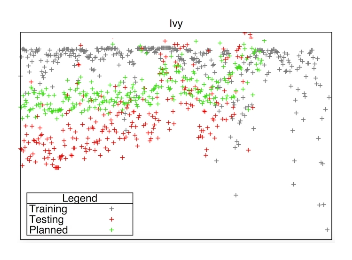
\includegraphics[width=\linewidth]{figs/2d.eps} 
%  % 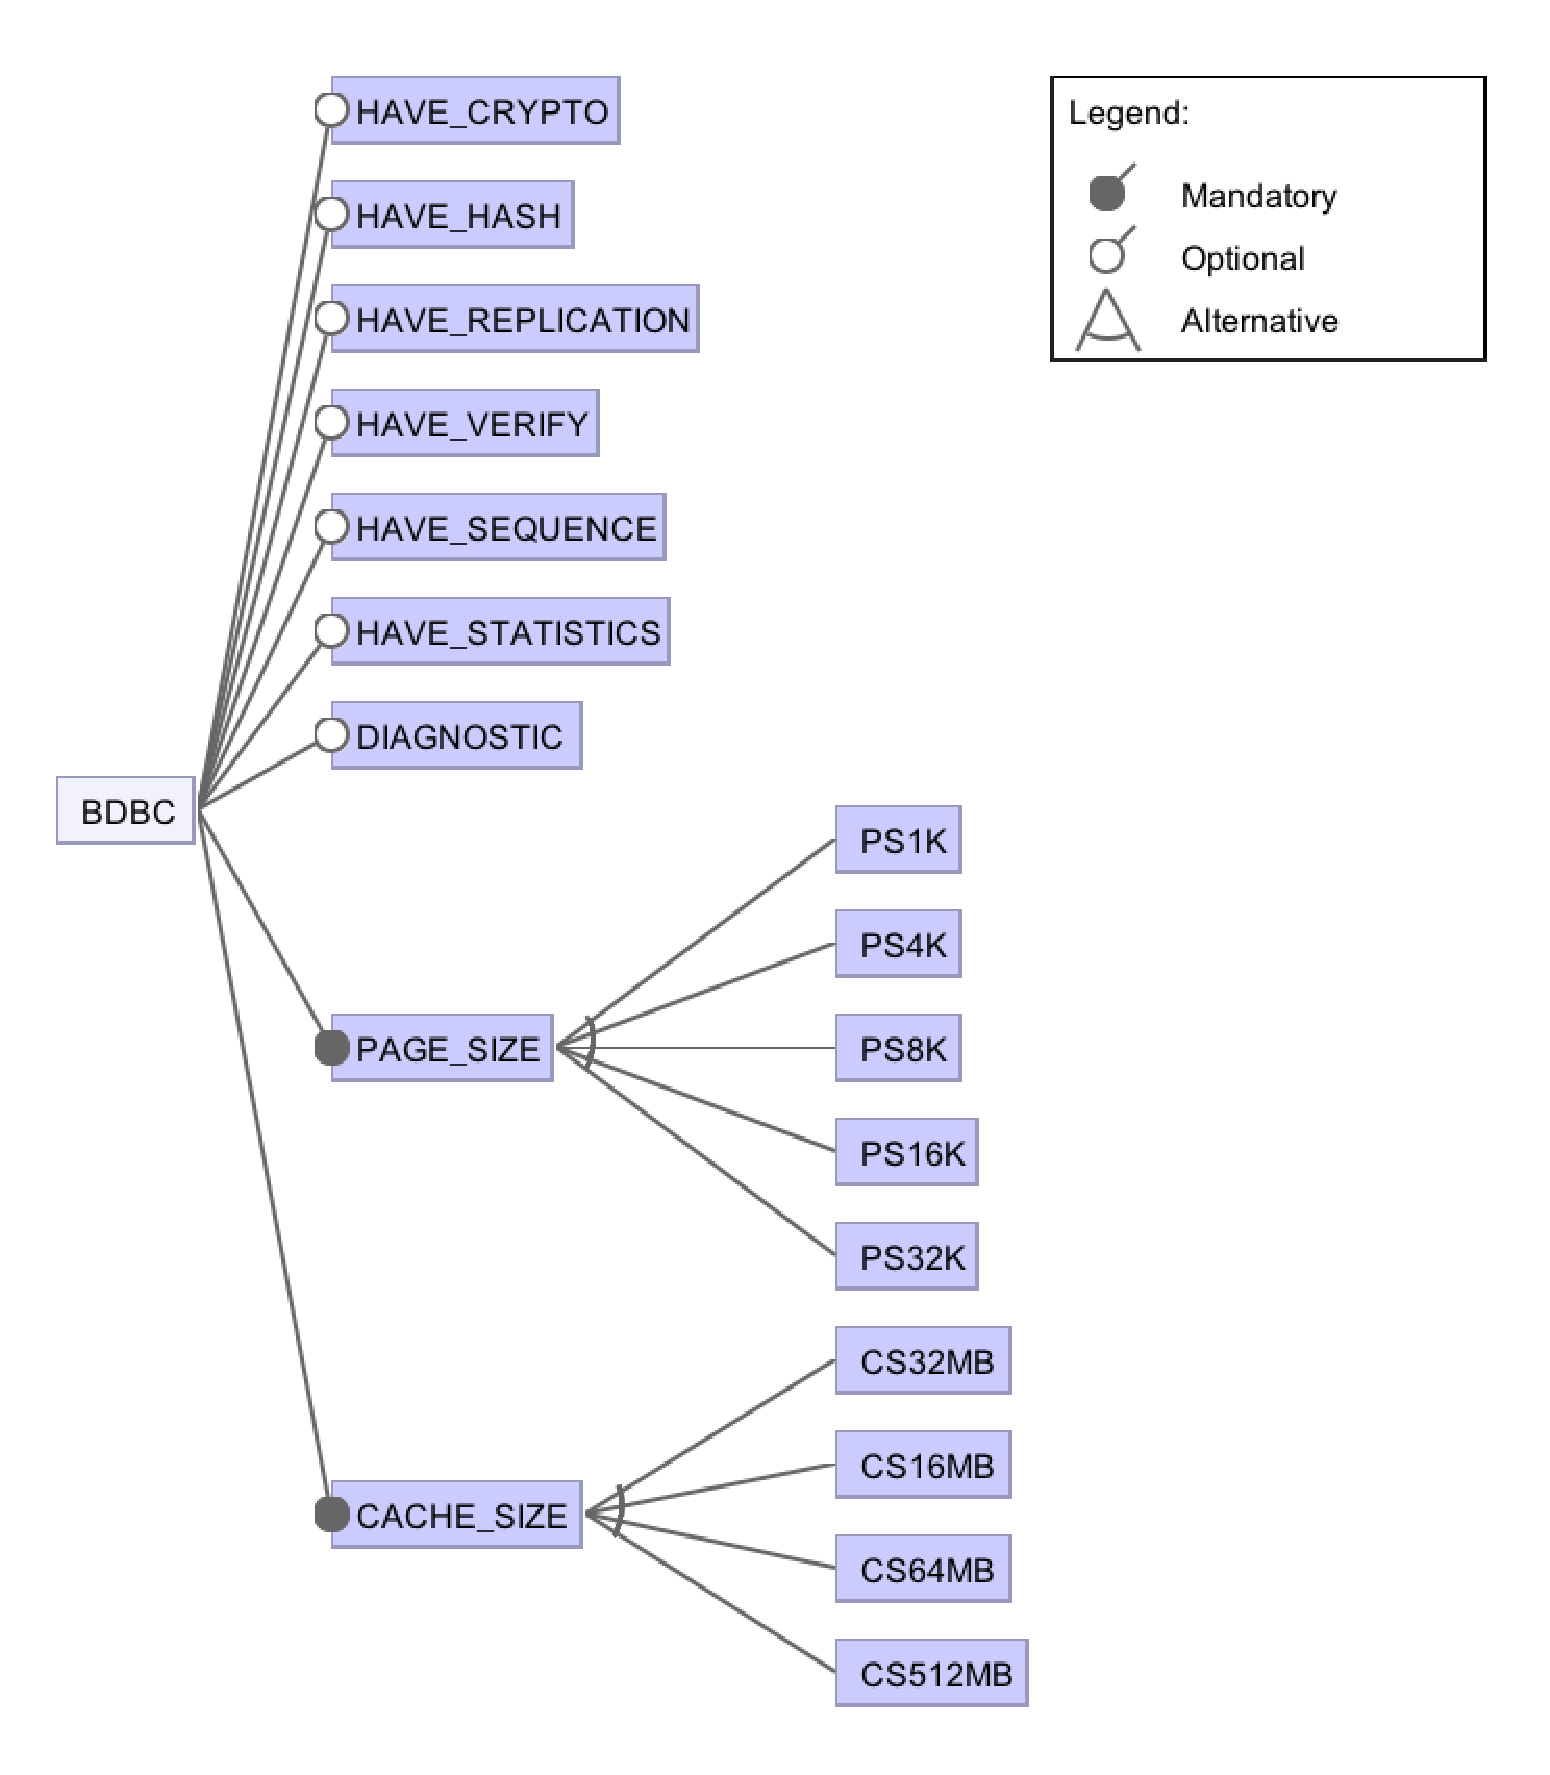
\includegraphics[width=1\linewidth]{figs/BDBC.eps}
% \caption{Gray, red, green show (1) training examples, (2) test examples and 
%   (3) tests that have been altered by planners.
%   This figure uses axes generated from the first two components of a PCA analysis of all points. 
% }\label{fig:howxy}
% \end{figure}
% We should mistrust the predictions made by a  model   if it is being applied to examples  that are
% too far away from the
% training cloud.
% To test for ``too far'', we can run a data mining experiment that tests how well
% a model learned from the training data applies to the test data. Such experiments return some performance value.

% Note that predictions  about changes that  fall within the space of the training+test data, will be at least
% as accurate as the predictions of the original test data. With this, we assert that the predictions for changes that move examples towards/away from the training data can be trusted more/less (respectively).

% Accordingly, we need {\em trust-increasing} planners to generate new examples {\em closer} to the
% training examples.  To see how this works, 
%  \fig{howxy} is from the {\em ivy} data
% set (one of the Jureczko data sets used in this paper). It shows: (1)~the training examples in gray, (2)~the test examples in red, and (3)~the
% changed  examples displaced after applying a plan (in green).
%  Note that the  the   changed examples
% cases  (shown in green)  fall closer to the training cases (shown in gray) than
% the test cases (shown in red). 

% In that green region of changed examples, our belief in the value of predictions
% will be just as much as, if not more than, our belief in the value of the predictions in the red region (that
% contains the original test data).
% This pattern of \fig{howxy} (where the new examples are found closer to  the training cases than the test cases) has been observed in all the other data sets studied in this
% paper. Hence,  we can assert that
% predictors learned from these training examples have some authority in the regions
% containing the changes examples.


% That said, the above comes with some important caveats:
% \bi
% \item 
% The quality of the prediction depends on the nature of the training data. Thus, we strongly recommend that both the data set and the predictor be assessed prior to planning. This ensures that the predictor's performance is adequate for a data set. We tackle this issue in detail in \tion{tesd}.
% \item
% Planners should be designed to be {\em trust increasing}. We list four such planning methods in \tion{planners}.
% \item
% Where possible, planners should be assessed via some external
% oracle that can accurately assess new examples. For an example of that kind of analysis,
% see  \tion{coc}.
% \ei

\subsection{  Internal Validity}\label{sect:coc}

% The main internal validity threat   in this study was the use of
% optimistic reasoning when generating the changed code modules.
We assumed in \tion{rq}
that any code module can be changed in order
to stop triggering a bad smell detector. This is not necessarily
true, as noted in {\em PROBLEM \#2} in this paper's introduction.
To mitigate this issue:
\begin{itemize}
    \item We do not propose using XTREE as a bad
smell generator;
\item Rather, we offer it as  a critique agent for bad smells
proposed by some other oracle (e.g. a human developer).
\end{itemize}
We showed about that XTREE's recommendations are not verbose.
That is, even if XTREE recommends the superset of possibly important bad smells,
that superset is not so large as to  overlap with many
 bad smell proposed at random 
by   developers. 

XTREE does not require a working defect predictor to generate
its bad smell thresholds. However, to {\em certify}
that those thresholds are satisfactory, some
second quality predictor must be applied. A data set containing defect counts before and after refactoring activities would enable an accurate assessment of the performance of the threshold-setting and recommender methods, however, such a data set is not available at this time.

 Historically,
SE researchers~\cite{Cheng10,OKeeffe08,OKeeffe07,Moghadam2011,Mkaouer14} have used the QMOOD hierarchical quality model~\cite{Bansiya02}.
Since such quality models may be very project specific~\cite{localvsglobal}, we prefer building local 
defect predictors using Random Forests. We chose this approach,  based on its reputation for having the better  performance of 21 other learners for defect prediction~\cite{lessmann}.  
Our results show that when a defect log contains too few
non-defective examples then defector predictors
perform poorly (see the data sets in the last few lines of \fig{j})
as do their associated bad smell threshold generators
(recall the performance of Lucene and Poi in~\fig{jur}). It should be noted that this is not a limitation of XTREE-- rather
it seems fundamental to the problem of certifying bad smells.
As evidence of this, recall that {\em all} the bad smell threshold generators of~\fig{jur}
had issues with the defect data sets with  many defects
(Lucene and Poi).


% \subsection{ Learner Bias}
% This study used two kinds of learners: (1) methods for suggesting
% changes to code like Shatnawi, Alves et al., CD and XTREE;
% (2) methods for assessing the changes proposed by these learners.
% Prior studies implemented (2) using  the QMOOD hierarchical quality model
% which is so old, that we suspect it may no longer be current. Hence,
% we used Random Forests to build the assessment oracles that were specific
% to the data sets used in this study. We chose this approach,  based on its reputation for having the better  performance of 21 other learners for defect prediction~\cite{lessmann}. 

  



% \subsection{  Sampling bias} 
% Sampling bias threatens any data mining experiment; i.e., what matters
% there may not be true here. For example, the data sets used here comes from two  Jureczko et al. and any biases in their selection procedures
% threaten the validity of these results. 
% That said,
% the best we can do is define our methods and publicize our data and code so that other researchers can
% try to repeat our results and, perhaps, point out a previously unknown bias
% in our analysis. Hopefully, other researchers will emulate our methods in
% order to repeat, refute, or improve our results. 





% \begin{figure}[!t]
%\noindent\begin{minipage}{0.5\textwidth} 
{\small 
\begin{tabular}{llrrc}
\arrayrulecolor{lightgray}
\rowcolor{lightgray}\textbf{Rank} & \textbf{Treatment} & \textbf{Median} & \textbf{IQR} & \\\hline
  1 &        XTREE &   59   &  9 & \quart{75}{4}{78}{99} \\
2 &      CD &    -9  &  77 & \quart{21}{41}{42}{99} \\
\hline \end{tabular}}
\caption{Planners applied to some ground-truth data (in this case, the POM3 model).
Values collected from  40 repeated runs of each method with different random seeds.
Results show the efficacy of XTREE in reducing the total overall cost in the original test data, when CD fail to do so.}
\label{fig:coc}
\end{figure}


\section{Conclusions}
Which  bad smells can  be ignored? 
We say: ignore those not supported by the historical log of data from
the current project.  

When that data is not available (e.g. early
in the project) then developers could use the general list of
bad smells shown in \fig{smells}. However, 
our results
show that  bad smell detectors are most
effective when they are based
on a small handful of code metrics (as done by XTREE).
Hence, using all the bad smells of \fig{smells} may not be optimal.

XTREE improves on prior methods for generating bad smells:
\begin{itemize}
    \item As described in \tion{prelim}, bad smells generated by humans may not be applicable to the current project. On the other hand, XTREE can automatically learn specific thresholds
    for bad smells for the current project.
    \item Prior methods used an old quality predictor (QMOOD) which we replace with defect predictors learned via Random Forests
    from   current project data.
    \item As described in in \tion{bst}, 
    XTREE generates conjunctions of code metric thresholds
    that need to be satisfied at the same time.
    Older methods, such as those proposed by  Shatnawi and Alves
    offer only disjunctions that might be inappropriately applied
    to yield impossible refactorings (e.g. reducing lines of code
    and coupling at the same time).
    
    \item XTREE's conjunctions proved to be arguably as effective
    as those of Alves (see \fig{jur}) but far less verbose (see \fig{counts}) thus making XTREE a better tool for critiquing and rejecting
    more bad smells proposed by developers.
\end{itemize}
In summary, this paper offers a baseline result
that XTREE can be used as a {\em diagnostic tool}
for identifying which bad smells can be ignored.
But can it be used as a {\em prescriptive tool}
to recommend new refactorings?  

As discussed in {\em PROBLEM \#2}
(from the introduction), XTREE might propose
changes to code metrics that are
not feasible  (due to the local domain constraints
of the code). To repair this, XTREE needs to be extended
with architectural knowledge of the code it is studying.
Elsewhere, we have had some   success
with reasoning about such architectural knowledge
(expressed as software product lines~\cite{sayyad13a,sayyad13b}). In future
work, we will explore extending XTREE 
with  
architectural knowledge such that it can
become a tool which perscribes
feasible refactorings. 


\section*{Acknowledgements}
The work is partially funded by NSF  awards \#1506586 and \#1302169.

% \bibliographystyle{plain}
\balance
\bibliographystyle{unsrt}
\bibliography{References}
\end{document}